% Skill or state machine? Guidance versus control for LLM research agents on miRNA-target prediction.
% Laid out like the Agentomics-ML preprint (NeurIPS preprint style): Times text, Computer Modern maths, booktabs tables.
% Build: `make` (runs generate.py, then latexmk; see latexmkrc). Every number, table and chart series comes from
% data/report-data.json through generated.tex; sections/ holds the text, figures/ the TikZ drawings and plots.
\documentclass[10pt]{article}

% ── Page and fonts: as the NeurIPS preprint style ──
\usepackage[letterpaper, textwidth=5.5in, textheight=9in, top=1in, headheight=12pt, headsep=25pt, footskip=30pt]{geometry}
\usepackage[T1]{fontenc}
\usepackage[utf8]{inputenc}
\usepackage{times}
\usepackage{microtype}
\usepackage{amsmath,amssymb}

% ── Tables, figures, lists ──
\usepackage{booktabs,longtable,array}
\usepackage{xcolor}
\usepackage{caption}
\usepackage{subcaption}
\usepackage{float}
\usepackage{listings}
\lstset{basicstyle=\ttfamily\scriptsize, breaklines=true, columns=fullflexible, frame=tb, framerule=0.4pt,
  aboveskip=0.8em, xleftmargin=0pt, extendedchars=true, inputencoding=utf8,
  literate={├}{{|-}}2 {└}{{`-}}2 {─}{{-}}1 {…}{{...}}3}
\usepackage{pgfplots}
\usepgfplotslibrary{groupplots}
\usetikzlibrary{arrows.meta, positioning, calc, patterns}
\pgfplotsset{compat=1.18}

% ── References and links ──
\usepackage[round, authoryear]{natbib}
\usepackage{url}
\usepackage{hyperref}
\hypersetup{hidelinks, pdftitle={Skill or State Machine? Guidance versus Control for LLM Research Agents on miRNA-Target Prediction},
  pdfauthor={Vlastimil Martinek, Andrea Gariboldi, Dimosthenis Tzimotoudis, Mark Galea, Elissavet Zacharopoulou, Panagiotis Alexiou}}
\usepackage[capitalise, noabbrev]{cleveref}

% ── Colours: only the charts tell the two methods apart ──
\definecolor{skill}{HTML}{0F7B6C}
\definecolor{sm}{HTML}{4B4FB8}
\definecolor{seg1}{HTML}{7AA6C2}\definecolor{seg2}{HTML}{4B7FA3}\definecolor{seg3}{HTML}{2C5878}
\definecolor{seg4}{HTML}{1D3C55}\definecolor{seg5}{HTML}{142B3D}
\pgfplotsset{every axis/.append style={tick label style={font=\footnotesize}, label style={font=\small}}}
\pgfplotsset{skill/.style={color=skill,thick}, sm/.style={color=sm,thick}}

% ── Text block: no indent, space between paragraphs ──
\setlength{\parindent}{0pt}
\setlength{\parskip}{5.5pt}
\setlength{\emergencystretch}{1.5em}
\widowpenalty=10000
\clubpenalty=10000
\captionsetup{labelsep=colon, skip=6pt}
\captionsetup[table]{position=top}
\newcommand{\vs}{ vs.\ }

% ── Headings: as the NeurIPS style (bold serif, numbered) ──
\makeatletter
\renewcommand{\section}{\@startsection{section}{1}{\z@}{-2.0ex \@plus -0.5ex \@minus -0.2ex}{1.5ex \@plus 0.3ex \@minus 0.2ex}{\large\bfseries\raggedright}}
\renewcommand{\subsection}{\@startsection{subsection}{2}{\z@}{-1.8ex \@plus -0.5ex \@minus -0.2ex}{0.8ex \@plus 0.2ex}{\normalsize\bfseries\raggedright}}
\renewcommand{\paragraph}{\@startsection{paragraph}{4}{\z@}{1.5ex \@plus 0.5ex \@minus 0.2ex}{-1em}{\normalsize\bfseries}}
\makeatother

% Let a page take more float material before LaTeX moves floats to a page of their own.
\renewcommand{\topfraction}{0.9}\renewcommand{\bottomfraction}{0.8}\renewcommand{\textfraction}{0.07}
\renewcommand{\floatpagefraction}{0.8}\setcounter{topnumber}{3}\setcounter{bottomnumber}{2}\setcounter{totalnumber}{4}

\newcommand{\SkillCost}{\$53.16}
\newcommand{\SkillTime}{4.4\,h}
\newcommand{\SmCost}{\$141.25}
\newcommand{\SmTime}{17.0\,h}
\newcommand{\BestScore}{0.912}
\newcommand{\BestCell}{Claude Fable 5.2, state machine, reasoning \texttt{none}}
\newcommand{\SkillCalls}{890}
\newcommand{\SmCalls}{3{,}590}
\newcommand{\HighWins}{13}
\newcommand{\HighPairs}{18}
\newcommand{\ScoredRuns}{36}
\newcommand{\FlagSkillAvgCost}{\$5.11}
\newcommand{\FlagSmAvgCost}{\$14.64}
\newcommand{\SmallSkillAvgCost}{\$1.23}
\newcommand{\SmallSmAvgCost}{\$2.41}
\newcommand{\CostRatio}{38\%}
\newcommand{\TimeRatio}{26\%}
\newcommand{\SkillMean}{0.831}\newcommand{\SkillMedian}{0.862}\newcommand{\SkillBest}{0.910}
\newcommand{\SkillAboveAgentomics}{14}\newcommand{\SkillAboveSota}{9}
\newcommand{\SmMean}{0.845}\newcommand{\SmMedian}{0.885}\newcommand{\SmBest}{0.912}
\newcommand{\SmAboveAgentomics}{13}\newcommand{\SmAboveSota}{12}
\newcommand{\GptSmNone}{0.666}\newcommand{\GptSmHigh}{0.726}\newcommand{\GptSmMean}{0.696}\newcommand{\GptSmBest}{0.726}
\newcommand{\GptSkillNone}{0.781}\newcommand{\GptSkillHigh}{0.754}\newcommand{\GptSkillMean}{0.767}\newcommand{\GptSkillBest}{0.781}
\newcommand{\WilcoxonP}{0.32}
\newcommand{\WilcoxonN}{18}
\newcommand{\MedianDiff}{0.004}
\newcommand{\CIHalfMed}{0.025}
\newcommand{\PairsSm}{7}
\newcommand{\PairsSkill}{2}
\newcommand{\PairsTie}{9}
\newcommand{\FlagHighTies}{4}
\newcommand{\FlagHighMax}{0.006}
\newcommand{\SmallSm}{5}
\newcommand{\SmallSkill}{2}
\newcommand{\FlagScoreMin}{0.844}
\newcommand{\FlagScoreMax}{0.912}
\newcommand{\SmallScoreMin}{0.666}
\newcommand{\SmallScoreMax}{0.907}
\newcommand{\SmallPairs}{10}
\newcommand{\PairTable}{%
\begin{tabular}{@{}l l r r r r l@{}}\toprule
\textbf{Model} & \textbf{Reas.} & \textbf{Skill} & \textbf{SM} & \textbf{$\Delta$} & \textbf{95\% CI} & \textbf{Winner}\\\midrule
\multicolumn{7}{@{}l}{\emph{Top-of-line models}}\\
Claude Fable 5.2 & none & 0.895 & \textbf{0.912}$^{\ddagger}$ & $\mathbf{+0.018}$ & $[+0.008,\;+0.027]$ & \textbf{SM}\\
Claude Fable 5.2 & high & 0.906 & 0.902$^{\ddagger}$ & $-0.004$ & $[-0.009,\;+0.001]$ & tie\\
\addlinespace[3pt]
Claude Opus 5.5 & none & 0.903 & 0.899$^{\dagger}$ & $-0.004$ & $[-0.015,\;+0.006]$ & tie\\
Claude Opus 5.5 & high & 0.910 & 0.907 & $-0.003$ & $[-0.014,\;+0.007]$ & tie\\
\addlinespace[3pt]
GPT-6.2 Astra & none & 0.844 & \textbf{0.890}$^{\ddagger}$ & $\mathbf{+0.046}$ & $[+0.027,\;+0.065]$ & \textbf{SM}\\
GPT-6.2 Astra & high & 0.903$^{\dagger}$ & 0.909$^{\dagger}$ & $+0.006$ & $[-0.004,\;+0.015]$ & tie\\
\addlinespace[3pt]
Gemini 4 Hydrogen & none & 0.886$^{\ddagger}$ & 0.880$^{\dagger}$ & $-0.006$ & $[-0.021,\;+0.010]$ & tie\\
Gemini 4 Hydrogen & high & 0.907 & 0.906$^{\ddagger}$ & $0.000$ & $[-0.007,\;+0.007]$ & tie\\
\midrule
\multicolumn{7}{@{}l}{\emph{Mid-range models}}\\
Claude Sonnet 5.5 & none & 0.869 & 0.871$^{\dagger}$ & $+0.002$ & $[-0.021,\;+0.023]$ & tie\\
Claude Sonnet 5.5 & high & 0.868 & \textbf{0.903} & $\mathbf{+0.035}$ & $[+0.020,\;+0.050]$ & \textbf{SM}\\
\addlinespace[3pt]
Qwen 3.5 122B-A10B & none & \textbf{0.781} & 0.708$^{\ddagger}$ & $\mathbf{-0.073}$ & $[-0.114,\;-0.032]$ & \textbf{Skill}\\
Qwen 3.5 122B-A10B & high & 0.813 & 0.827$^{\ddagger}$ & $+0.014$ & $[-0.018,\;+0.047]$ & tie\\
\addlinespace[3pt]
Claude Haiku 4.5 & none & 0.680 & \textbf{0.775} & $\mathbf{+0.095}$ & $[+0.056,\;+0.136]$ & \textbf{SM}\\
Claude Haiku 4.5 & high & 0.674 & \textbf{0.739}$^{\ddagger}$ & $\mathbf{+0.065}$ & $[+0.031,\;+0.098]$ & \textbf{SM}\\
\addlinespace[3pt]
DeepSeek V4.1 Flash & none & 0.732 & \textbf{0.881}$^{\ddagger}$ & $\mathbf{+0.149}$ & $[+0.118,\;+0.181]$ & \textbf{SM}\\
DeepSeek V4.1 Flash & high & 0.856 & \textbf{0.907}$^{\ddagger}$ & $\mathbf{+0.050}$ & $[+0.027,\;+0.073]$ & \textbf{SM}\\
\addlinespace[3pt]
GPT-4.1 & none & \textbf{0.781}$^{\dagger}$ & 0.666$^{\dagger}$ & $\mathbf{-0.115}$ & $[-0.156,\;-0.069]$ & \textbf{Skill}\\
GPT-4.1 & high & 0.754$^{\dagger}$ & 0.726$^{\dagger}$ & $-0.027$ & $[-0.063,\;+0.007]$ & tie\\
\bottomrule\end{tabular}}
\newcommand{\PairTableNote}{\footnotesize SM: state machine wins; Skill: skill wins; tie: 95\% CI includes zero.}
\newcommand{\BestSkilla}{0.906}\newcommand{\BestSma}{0.912}
\newcommand{\BestSkillb}{0.910}\newcommand{\BestSmb}{0.907}
\newcommand{\BestSkillc}{0.903}\newcommand{\BestSmc}{0.909}
\newcommand{\BestSkilld}{0.907}\newcommand{\BestSmd}{0.906}
\newcommand{\BestSkille}{0.869}\newcommand{\BestSme}{0.903}
\newcommand{\BestSkillf}{0.813}\newcommand{\BestSmf}{0.827}
\newcommand{\BestSkillg}{0.680}\newcommand{\BestSmg}{0.775}
\newcommand{\BestSkillh}{0.856}\newcommand{\BestSmh}{0.907}
\newcommand{\BestSkilli}{0.781}\newcommand{\BestSmi}{0.726}
\newcommand{\MatrixTable}{%
\begin{tabular}{@{}l rr rr@{}}\toprule
& \multicolumn{2}{c}{\textbf{Skill}} & \multicolumn{2}{c}{\textbf{SM}}\\\cmidrule(lr){2-3}\cmidrule(l){4-5}\textbf{Model} & \textbf{none} & \textbf{high} & \textbf{none} & \textbf{high}\\\midrule
Claude Fable 5.2 & 0.895 & 0.906 & \underline{\textbf{0.912}}$^{\ddagger}$ & 0.902$^{\ddagger}$\\
Claude Opus 5.5 & 0.903 & \textbf{0.910} & 0.899$^{\dagger}$ & 0.907\\
GPT-6.2 Astra & 0.844 & 0.903$^{\dagger}$ & 0.890$^{\ddagger}$ & \textbf{0.909}$^{\dagger}$\\
Gemini 4 Hydrogen & 0.886$^{\ddagger}$ & \textbf{0.907} & 0.880$^{\dagger}$ & 0.906$^{\ddagger}$\\
Claude Sonnet 5.5 & 0.869 & 0.868 & 0.871$^{\dagger}$ & \textbf{0.903}\\
Qwen 3.5 122B-A10B & 0.781 & 0.813 & 0.708$^{\ddagger}$ & \textbf{0.827}$^{\ddagger}$\\
Claude Haiku 4.5 & 0.680 & 0.674 & \textbf{0.775} & 0.739$^{\ddagger}$\\
DeepSeek V4.1 Flash & 0.732 & 0.856 & 0.881$^{\ddagger}$ & \textbf{0.907}$^{\ddagger}$\\
GPT-4.1 & \textbf{0.781}$^{\dagger}$ & 0.754$^{\dagger}$ & 0.666$^{\dagger}$ & 0.726$^{\dagger}$\\
\midrule
Mean & 0.819 & 0.843 & 0.831 & 0.858\\
Median & 0.844 & 0.868 & 0.880 & 0.903\\
\bottomrule\end{tabular}}
\newcommand{\CostTable}{%
\begin{tabular}{@{}l rr rr@{}}\toprule
& \multicolumn{2}{c}{\textbf{Skill}} & \multicolumn{2}{c}{\textbf{SM}}\\\cmidrule(lr){2-3}\cmidrule(l){4-5}\textbf{Model} & \textbf{none} & \textbf{high} & \textbf{none} & \textbf{high}\\\midrule
Claude Fable 5.2 & \textbf{7.72} & 18.52 & 15.22 & 71.21\\
Claude Opus 5.5 & \textbf{1.57} & 10.14 & 3.44 & 16.17\\
GPT-6.2 Astra & \textbf{0.25} & 0.68 & 1.68 & 3.74\\
Gemini 4 Hydrogen & \textbf{0.39} & 1.63 & 0.73 & 4.94\\
Claude Sonnet 5.5 & 1.13 & \textbf{0.91} & 1.05 & 3.27\\
Qwen 3.5 122B-A10B & 0.45 & \textbf{0.29} & 2.89 & 2.25\\
Claude Haiku 4.5 & \textbf{1.27} & 1.83 & 3.98 & 6.44\\
DeepSeek V4.1 Flash & \underline{\textbf{0.05}} & 0.08 & 0.30 & 0.34\\
GPT-4.1 & 5.92 & \textbf{0.33} & 1.50 & 2.10\\
\midrule
Mean & 2.08 & 3.82 & 3.42 & 12.27\\
Median & 1.13 & 0.91 & 1.68 & 3.74\\
\bottomrule\end{tabular}}
\newcommand{\TimeTable}{%
\begin{tabular}{@{}l rr rr@{}}\toprule
& \multicolumn{2}{c}{\textbf{Skill}} & \multicolumn{2}{c}{\textbf{SM}}\\\cmidrule(lr){2-3}\cmidrule(l){4-5}\textbf{Model} & \textbf{none} & \textbf{high} & \textbf{none} & \textbf{high}\\\midrule
Claude Fable 5.2 & \textbf{32} & 34 & 109 & 175\\
Claude Opus 5.5 & \textbf{4} & 59 & 14 & 105\\
GPT-6.2 Astra & \underline{\textbf{1}} & 6 & 7 & 17\\
Gemini 4 Hydrogen & 18 & 22 & \textbf{10} & 62\\
Claude Sonnet 5.5 & 9 & \textbf{5} & 15 & 17\\
Qwen 3.5 122B-A10B & \textbf{4} & 7 & 36 & 24\\
Claude Haiku 4.5 & \textbf{5} & \textbf{5} & 20 & 25\\
DeepSeek V4.1 Flash & 30 & \textbf{14} & 148 & 80\\
GPT-4.1 & 5 & \textbf{2} & 57 & 102\\
\midrule
Mean & 12 & 17 & 46 & 67\\
Median & 5 & 7 & 20 & 62\\
\bottomrule\end{tabular}}
\newcommand{\FlagSmTierMean}{0.901}\newcommand{\FlagSmTierMedian}{0.904}\newcommand{\FlagSmTierBest}{0.912}\newcommand{\FlagSmTierRuns}{8}
\newcommand{\FlagSkillTierMean}{0.894}\newcommand{\FlagSkillTierMedian}{0.903}\newcommand{\FlagSkillTierBest}{0.910}\newcommand{\FlagSkillTierRuns}{8}
\newcommand{\MidSmTierMean}{0.800}\newcommand{\MidSmTierMedian}{0.801}\newcommand{\MidSmTierBest}{0.907}\newcommand{\MidSmTierRuns}{10}
\newcommand{\MidSkillTierMean}{0.781}\newcommand{\MidSkillTierMedian}{0.781}\newcommand{\MidSkillTierBest}{0.869}\newcommand{\MidSkillTierRuns}{10}
\newcommand{\FirstRuns}{35}
\newcommand{\FirstAboveSota}{13}
\newcommand{\FirstFlagGain}{0.051}
\newcommand{\FirstSmallGain}{0.143}
\newcommand{\FirstSkillMean}{0.704}
\newcommand{\FirstSmMean}{0.761}
\newcommand{\FirstGap}{0.057}
\newcommand{\FinalGap}{0.014}
\newcommand{\FirstPairTable}{%
\begin{tabular}{@{}l l r r r r l@{}}\toprule
\textbf{Model} & \textbf{Reas.} & \textbf{Skill} & \textbf{SM} & \textbf{$\Delta$} & \textbf{95\% CI} & \textbf{Winner}\\\midrule
\multicolumn{7}{@{}l}{\emph{Top-of-line models}}\\
Claude Fable 5.2 & none & 0.854 & \textbf{0.894}$^{\ddagger}$ & $\mathbf{+0.040}$ & $[+0.026,\;+0.056]$ & \textbf{SM}\\
Claude Fable 5.2 & high & 0.873 & \textbf{0.888}$^{\ddagger}$ & $\mathbf{+0.014}$ & $[+0.002,\;+0.028]$ & \textbf{SM}\\
\addlinespace[3pt]
Claude Opus 5.5 & none & \textbf{0.888} & 0.862$^{\dagger}$ & $\mathbf{-0.026}$ & $[-0.044,\;-0.010]$ & \textbf{Skill}\\
Claude Opus 5.5 & high & 0.886 & 0.891 & $+0.004$ & $[-0.010,\;+0.019]$ & tie\\
\addlinespace[3pt]
GPT-6.2 Astra & none & 0.695 & \textbf{0.830}$^{\ddagger}$ & $\mathbf{+0.135}$ & $[+0.104,\;+0.163]$ & \textbf{SM}\\
GPT-6.2 Astra & high & \textbf{0.875}$^{\dagger}$ & 0.764$^{\dagger}$ & $\mathbf{-0.111}$ & $[-0.139,\;-0.087]$ & \textbf{Skill}\\
\addlinespace[3pt]
Gemini 4 Hydrogen & none & N/A$^{\ddagger}$ & 0.754$^{\dagger}$ & -- & -- & --\\
Gemini 4 Hydrogen & high & 0.876 & 0.885$^{\ddagger}$ & $+0.009$ & $[0.000,\;+0.019]$ & tie\\
\midrule
\multicolumn{7}{@{}l}{\emph{Mid-range models}}\\
Claude Sonnet 5.5 & none & 0.824 & 0.816$^{\dagger}$ & $-0.008$ & $[-0.026,\;+0.009]$ & tie\\
Claude Sonnet 5.5 & high & 0.767 & \textbf{0.898} & $\mathbf{+0.131}$ & $[+0.105,\;+0.159]$ & \textbf{SM}\\
\addlinespace[3pt]
Qwen 3.5 122B-A10B & none & 0.650 & \textbf{0.708}$^{\ddagger}$ & $\mathbf{+0.058}$ & $[+0.013,\;+0.102]$ & \textbf{SM}\\
Qwen 3.5 122B-A10B & high & 0.447 & \textbf{0.789}$^{\ddagger}$ & $\mathbf{+0.342}$ & $[+0.294,\;+0.383]$ & \textbf{SM}\\
\addlinespace[3pt]
Claude Haiku 4.5 & none & 0.440 & 0.445 & $+0.005$ & $[-0.022,\;+0.033]$ & tie\\
Claude Haiku 4.5 & high & 0.438 & \textbf{0.576}$^{\ddagger}$ & $\mathbf{+0.138}$ & $[+0.092,\;+0.181]$ & \textbf{SM}\\
\addlinespace[3pt]
DeepSeek V4.1 Flash & none & 0.633 & \textbf{0.881}$^{\ddagger}$ & $\mathbf{+0.248}$ & $[+0.205,\;+0.289]$ & \textbf{SM}\\
DeepSeek V4.1 Flash & high & 0.848 & \textbf{0.907}$^{\ddagger}$ & $\mathbf{+0.058}$ & $[+0.035,\;+0.082]$ & \textbf{SM}\\
\addlinespace[3pt]
GPT-4.1 & none & \textbf{0.535}$^{\dagger}$ & 0.440$^{\dagger}$ & $\mathbf{-0.095}$ & $[-0.133,\;-0.056]$ & \textbf{Skill}\\
GPT-4.1 & high & 0.434$^{\dagger}$ & \textbf{0.473}$^{\dagger}$ & $\mathbf{+0.040}$ & $[+0.003,\;+0.076]$ & \textbf{SM}\\
\bottomrule\end{tabular}}
\newcommand{\FirstCiSm}{10}
\newcommand{\FirstCiSkill}{3}
\newcommand{\FirstCiTie}{4}
\newcommand{\FirstFlagCiSm}{3}
\newcommand{\FirstFlagCiPairs}{7}
\newcommand{\FirstMidCiSm}{7}
\newcommand{\FirstMidCiPairs}{10}
\newcommand{\FirstWilcoxonP}{=0.035}
\newcommand{\FirstMedianDiff}{0.040}
\newcommand{\FableSkillHighCost}{\$18.52}
\newcommand{\FableSmHighCost}{\$71.21}
\newcommand{\RunsCost}{\$194.41}
\newcommand{\SkillNoneMean}{0.819}
\newcommand{\SkillHighMean}{0.843}
\newcommand{\SmNoneMean}{0.831}
\newcommand{\SmHighMean}{0.858}
\newcommand{\SkillHighWins}{6}
\newcommand{\SmHighWins}{7}
\newcommand{\SkillReasonGain}{0.024}
\newcommand{\SmReasonGain}{0.027}
\newcommand{\BudgetTable}{\begin{tabular}{@{}l c r r r r@{}}\toprule
\textbf{Method} & \textbf{Iterations} & \textbf{Runs with a model} & \textbf{Mean test AU-PRC} & \textbf{Cost} & \textbf{Time}\\\midrule
Skill & 1 & 17 & 0.704 & 30\% & 27\%\\
 & 2 & 17 & 0.800 & 51\% & 49\%\\
 & 3 & 18 & 0.831 & 100\% & 100\%\\
\midrule
State machine & 1 & 18 & 0.761 & 21\% & 19\%\\
 & 2 & 18 & 0.832 & 66\% & 57\%\\
 & 3 & 18 & 0.845 & 100\% & 100\%\\
\bottomrule\end{tabular}}
\newcommand{\TwoRuns}{35}
\newcommand{\TwoWithin}{19}
\newcommand{\TwoLoss}{0.020}
\newcommand{\TwoCostShare}{62}
\newcommand{\TwoTimeShare}{55}
\pgfplotsset{dotrows/.style={ytick={9,8,7,6,5,4,3,2,1}, yticklabels={{Claude Fable 5.2},{Claude Opus 5.5},{GPT-6.2 Astra},{Gemini 4 Hydrogen},{Claude Sonnet 5.5},{Qwen 3.5 122B-A10B},{Claude Haiku 4.5},{DeepSeek V4.1 Flash},{GPT-4.1}}}}
\newcommand{\DotPlots}{%
\addplot[skill, mark=o, error bars/.cd, x dir=both, x explicit, error mark=none, error bar style={line width=0.55pt, opacity=0.55}] coordinates {(0.8945,8.81) += (0.0212,0) -= (0.0235,0) (0.9029,7.81) += (0.0199,0) -= (0.0217,0) (0.8441,6.81) += (0.0286,0) -= (0.0295,0) (0.8863,5.81) += (0.0237,0) -= (0.0258,0) (0.8694,4.81) += (0.0250,0) -= (0.0270,0) (0.7805,3.81) += (0.0387,0) -= (0.0387,0) (0.6800,2.81) += (0.0449,0) -= (0.0452,0) (0.7319,1.81) += (0.0373,0) -= (0.0395,0) (0.7810,0.81) += (0.0356,0) -= (0.0388,0)};
\addplot[skill, mark=*, error bars/.cd, x dir=both, x explicit, error mark=none, error bar style={line width=0.55pt, opacity=0.55}] coordinates {(0.9063,8.94) += (0.0184,0) -= (0.0206,0) (0.9100,7.94) += (0.0190,0) -= (0.0217,0) (0.9030,6.94) += (0.0195,0) -= (0.0224,0) (0.9065,5.94) += (0.0193,0) -= (0.0206,0) (0.8681,4.94) += (0.0245,0) -= (0.0266,0) (0.8132,3.94) += (0.0340,0) -= (0.0382,0) (0.6739,2.94) += (0.0465,0) -= (0.0436,0) (0.8565,1.94) += (0.0280,0) -= (0.0301,0) (0.7537,0.94) += (0.0389,0) -= (0.0405,0)};
\addplot[sm, mark=square, error bars/.cd, x dir=both, x explicit, error mark=none, error bar style={line width=0.55pt, opacity=0.55}] coordinates {(0.9121,9.06) += (0.0181,0) -= (0.0196,0) (0.8986,8.06) += (0.0205,0) -= (0.0227,0) (0.8902,7.06) += (0.0224,0) -= (0.0243,0) (0.8803,6.06) += (0.0228,0) -= (0.0253,0) (0.8712,5.06) += (0.0271,0) -= (0.0305,0) (0.7080,4.06) += (0.0435,0) -= (0.0443,0) (0.7752,3.06) += (0.0346,0) -= (0.0403,0) (0.8805,2.06) += (0.0243,0) -= (0.0250,0) (0.6662,1.06) += (0.0498,0) -= (0.0444,0)};
\addplot[sm, mark=square*, error bars/.cd, x dir=both, x explicit, error mark=none, error bar style={line width=0.55pt, opacity=0.55}] coordinates {(0.9022,9.19) += (0.0194,0) -= (0.0217,0) (0.9068,8.19) += (0.0202,0) -= (0.0223,0) (0.9087,7.19) += (0.0194,0) -= (0.0207,0) (0.9063,6.19) += (0.0191,0) -= (0.0223,0) (0.9031,5.19) += (0.0202,0) -= (0.0224,0) (0.8268,4.19) += (0.0308,0) -= (0.0353,0) (0.7393,3.19) += (0.0396,0) -= (0.0420,0) (0.9066,2.19) += (0.0190,0) -= (0.0231,0) (0.7263,1.19) += (0.0452,0) -= (0.0452,0)};
}
\newcommand{\IterPlots}{%
\nextgroupplot[title={Claude Fable 5.2}, ylabel={test AU-PRC}, legend to name=iterlegend, legend columns=4, legend style={font=\footnotesize, draw=black!20, /tikz/every even column/.append style={column sep=0.6em}}]
\addplot[skill,densely dashed,mark=o] coordinates {(0.930,0.8536) (1.930,0.8945) (2.930,0.8945)};
\addlegendentry{skill (\texttt{none})}
\addplot[skill,solid,mark=*] coordinates {(0.975,0.8731) (1.975,0.8994) (2.975,0.9063)};
\addlegendentry{skill (\texttt{high})}
\addplot[sm,densely dashed,mark=square] coordinates {(1.025,0.8939) (2.025,0.9039) (3.025,0.9121)};
\addlegendentry{SM (\texttt{none})}
\addplot[sm,solid,mark=square*] coordinates {(1.070,0.8876) (2.070,0.9022) (3.070,0.9022)};
\addlegendentry{SM (\texttt{high})}
\draw[black!55, line width=0.5pt, densely dotted] (axis cs:0.7,0.860) -- (axis cs:3.3,0.860);
\nextgroupplot[title={Claude Opus 5.5}]
\addplot[skill,densely dashed,mark=o] coordinates {(0.930,0.8879) (1.930,0.9051) (2.930,0.9029)};
\addplot[skill,solid,mark=*] coordinates {(0.975,0.8861) (1.975,0.8957) (2.975,0.9100)};
\addplot[sm,densely dashed,mark=square] coordinates {(1.025,0.8620) (2.025,0.8640) (3.025,0.8986)};
\addplot[sm,solid,mark=square*] coordinates {(1.070,0.8905) (2.070,0.9019) (3.070,0.9068)};
\draw[black!55, line width=0.5pt, densely dotted] (axis cs:0.7,0.860) -- (axis cs:3.3,0.860);
\nextgroupplot[title={GPT-6.2 Astra}]
\addplot[skill,densely dashed,mark=o] coordinates {(0.930,0.6947) (1.930,0.8441) (2.930,0.8441)};
\addplot[skill,solid,mark=*] coordinates {(0.975,0.8755) (1.975,0.9056) (2.975,0.9030)};
\addplot[sm,densely dashed,mark=square] coordinates {(1.025,0.8296) (2.025,0.8859) (3.025,0.8902)};
\addplot[sm,solid,mark=square*] coordinates {(1.070,0.7643) (2.070,0.8947) (3.070,0.9087)};
\draw[black!55, line width=0.5pt, densely dotted] (axis cs:0.7,0.860) -- (axis cs:3.3,0.860);
\nextgroupplot[title={Gemini 4 Hydrogen}, ylabel={test AU-PRC}]
\addplot[skill,solid,mark=*] coordinates {(0.975,0.8762) (1.975,0.9001) (2.975,0.9065)};
\addplot[sm,densely dashed,mark=square] coordinates {(1.025,0.7542) (2.025,0.7542) (3.025,0.8803)};
\addplot[sm,solid,mark=square*] coordinates {(1.070,0.8850) (2.070,0.8994) (3.070,0.9063)};
\draw[black!55, line width=0.5pt, densely dotted] (axis cs:0.7,0.860) -- (axis cs:3.3,0.860);
\nextgroupplot[title={Claude Sonnet 5.5}]
\addplot[skill,densely dashed,mark=o] coordinates {(0.930,0.8240) (1.930,0.8672) (2.930,0.8694)};
\addplot[skill,solid,mark=*] coordinates {(0.975,0.7667) (1.975,0.8604) (2.975,0.8681)};
\addplot[sm,densely dashed,mark=square] coordinates {(1.025,0.8159) (2.025,0.8712) (3.025,0.8712)};
\addplot[sm,solid,mark=square*] coordinates {(1.070,0.8978) (2.070,0.9031) (3.070,0.9031)};
\draw[black!55, line width=0.5pt, densely dotted] (axis cs:0.7,0.860) -- (axis cs:3.3,0.860);
\nextgroupplot[title={Qwen 3.5 122B-A10B}]
\addplot[skill,densely dashed,mark=o] coordinates {(0.930,0.6504) (1.930,0.7805) (2.930,0.7805)};
\addplot[skill,solid,mark=*] coordinates {(0.975,0.4470) (1.975,0.8132) (2.975,0.8132)};
\addplot[sm,densely dashed,mark=square] coordinates {(1.025,0.7080) (2.025,0.7080) (3.025,0.7080)};
\addplot[sm,solid,mark=square*] coordinates {(1.070,0.7892) (2.070,0.8031) (3.070,0.8268)};
\draw[black!55, line width=0.5pt, densely dotted] (axis cs:0.7,0.860) -- (axis cs:3.3,0.860);
\nextgroupplot[title={Claude Haiku 4.5}, ylabel={test AU-PRC}, xlabel={iterations}]
\addplot[skill,densely dashed,mark=o] coordinates {(0.930,0.4398) (1.930,0.6716) (2.930,0.6800)};
\addplot[skill,solid,mark=*] coordinates {(0.975,0.4376) (1.975,0.6739) (2.975,0.6739)};
\addplot[sm,densely dashed,mark=square] coordinates {(1.025,0.4452) (2.025,0.7374) (3.025,0.7752)};
\addplot[sm,solid,mark=square*] coordinates {(1.070,0.5757) (2.070,0.7393) (3.070,0.7393)};
\draw[black!55, line width=0.5pt, densely dotted] (axis cs:0.7,0.860) -- (axis cs:3.3,0.860);
\nextgroupplot[title={DeepSeek V4.1 Flash}, xlabel={iterations}]
\addplot[skill,densely dashed,mark=o] coordinates {(0.930,0.6328) (1.930,0.6328) (2.930,0.7319)};
\addplot[skill,solid,mark=*] coordinates {(0.975,0.8484) (1.975,0.8469) (2.975,0.8565)};
\addplot[sm,densely dashed,mark=square] coordinates {(1.025,0.8810) (2.025,0.8808) (3.025,0.8805)};
\addplot[sm,solid,mark=square*] coordinates {(1.070,0.9066)};
\draw[black!55, line width=0.5pt, densely dotted] (axis cs:0.7,0.860) -- (axis cs:3.3,0.860);
\nextgroupplot[title={GPT-4.1}, xlabel={iterations}]
\addplot[skill,densely dashed,mark=o] coordinates {(0.930,0.5346) (1.930,0.7799) (2.930,0.7810)};
\addplot[skill,solid,mark=*] coordinates {(0.975,0.4336) (1.975,0.4336) (2.975,0.7537)};
\addplot[sm,densely dashed,mark=square] coordinates {(1.025,0.4397) (2.025,0.6662)};
\addplot[sm,solid,mark=square*] coordinates {(1.070,0.4732) (2.070,0.7522) (3.070,0.7263)};
\draw[black!55, line width=0.5pt, densely dotted] (axis cs:0.7,0.860) -- (axis cs:3.3,0.860);
}
\newcommand{\IterMeanPlots}{%
\nextgroupplot[title={Top-of-line models}, xlabel={iterations}, ylabel={mean test AU-PRC}, legend to name=itermeanlegend, legend columns=4, legend style={font=\footnotesize, draw=black!20, /tikz/every even column/.append style={column sep=0.6em}}]
\addplot[skill,densely dashed,mark=o] coordinates {(1,0.8121) (2,0.8813) (3,0.8805)};
\addlegendentry{skill (\texttt{none})}
\addplot[skill,solid,mark=*] coordinates {(1,0.8777) (2,0.9002) (3,0.9065)};
\addlegendentry{skill (\texttt{high})}
\addplot[sm,densely dashed,mark=square] coordinates {(1,0.8349) (2,0.8520) (3,0.8953)};
\addlegendentry{SM (\texttt{none})}
\addplot[sm,solid,mark=square*] coordinates {(1,0.8569) (2,0.8995) (3,0.9060)};
\addlegendentry{SM (\texttt{high})}
\draw[black!55, line width=0.5pt, densely dotted] (axis cs:0.7,0.860) -- (axis cs:3.3,0.860);
\nextgroupplot[title={Mid-range models}, xlabel={iterations}]
\addplot[skill,densely dashed,mark=o] coordinates {(1,0.6163) (2,0.7464) (3,0.7686)};
\addplot[skill,solid,mark=*] coordinates {(1,0.5867) (2,0.7256) (3,0.7931)};
\addplot[sm,densely dashed,mark=square] coordinates {(1,0.6580) (2,0.7727) (3,0.7802)};
\addplot[sm,solid,mark=square*] coordinates {(1,0.7285) (2,0.8209) (3,0.8204)};
\draw[black!55, line width=0.5pt, densely dotted] (axis cs:0.7,0.860) -- (axis cs:3.3,0.860);
\node[font=\scriptsize, text=black!60, anchor=south east] at (axis cs:3.28,0.860) {human state of the art};
}
\newcommand{\IterTable}[1]{%
\begin{longtable}{@{}l l l r r r r c r@{}}\caption{#1}\\\toprule
\textbf{Model} & \textbf{Method} & \textbf{Reas.} & \textbf{After 1} & \textbf{After 2} & \textbf{After 3} & \textbf{Final} & \textbf{Picked} & \textbf{Best on test}\\\midrule\endfirsthead
\toprule \textbf{Model} & \textbf{Method} & \textbf{Reas.} & \textbf{After 1} & \textbf{After 2} & \textbf{After 3} & \textbf{Final} & \textbf{Picked} & \textbf{Best on test}\\\midrule\endhead
Claude Fable 5.2 & Skill & none & 0.854 & 0.895 & 0.895 & 0.895 & 2 & \textbf{3 (0.901)}\\
Claude Fable 5.2 & Skill & high & 0.873 & 0.899 & 0.906 & 0.906 & 3 & 3 (0.906)\\
Claude Fable 5.2$^{\ddagger}$ & State machine & none & 0.894 & 0.904 & 0.912 & 0.912 & 3 & 3 (0.912)\\
Claude Fable 5.2$^{\ddagger}$ & State machine & high & 0.888 & 0.902 & 0.902 & 0.902 & 2 & 2 (0.902)\\
\midrule
Claude Opus 5.5 & Skill & none & 0.888 & 0.905 & 0.903 & 0.903 & 3 & \textbf{2 (0.905)}\\
Claude Opus 5.5 & Skill & high & 0.886 & 0.896 & 0.910 & 0.910 & 3 & 3 (0.910)\\
Claude Opus 5.5$^{\dagger}$ & State machine & none & 0.862 & 0.864 & 0.899 & 0.899 & 3 & 3 (0.899)\\
Claude Opus 5.5 & State machine & high & 0.891 & 0.902 & 0.907 & 0.907 & 3 & 3 (0.907)\\
\midrule
GPT-6.2 Astra & Skill & none & 0.695 & 0.844 & 0.844 & 0.844 & 2 & 2 (0.844)\\
GPT-6.2 Astra$^{\dagger}$ & Skill & high & 0.875 & 0.906 & 0.903 & 0.903 & 3 & \textbf{2 (0.906)}\\
GPT-6.2 Astra$^{\ddagger}$ & State machine & none & 0.830 & 0.886 & 0.890 & 0.890 & 3 & 3 (0.890)\\
GPT-6.2 Astra$^{\dagger}$ & State machine & high & 0.764 & 0.895 & 0.909 & 0.909 & 3 & 3 (0.909)\\
\midrule
Gemini 4 Hydrogen$^{\ddagger}$ & Skill & none & N/A & N/A & N/A & 0.886 & 5 & 5 (0.886)\\
Gemini 4 Hydrogen & Skill & high & 0.876 & 0.900 & 0.907 & 0.907 & 3 & 3 (0.907)\\
Gemini 4 Hydrogen$^{\dagger}$ & State machine & none & 0.754 & 0.754 & 0.880 & 0.880 & 3 & 3 (0.880)\\
Gemini 4 Hydrogen$^{\ddagger}$ & State machine & high & 0.885 & 0.899 & 0.906 & 0.906 & 3 & 3 (0.906)\\
\midrule
Claude Sonnet 5.5 & Skill & none & 0.824 & 0.867 & 0.869 & 0.869 & 3 & 3 (0.869)\\
Claude Sonnet 5.5 & Skill & high & 0.767 & 0.860 & 0.868 & 0.868 & 3 & 3 (0.868)\\
Claude Sonnet 5.5$^{\dagger}$ & State machine & none & 0.816 & 0.871 & 0.871 & 0.871 & 2 & 2 (0.871)\\
Claude Sonnet 5.5 & State machine & high & 0.898 & 0.903 & 0.903 & 0.903 & 2 & \textbf{3 (0.904)}\\
\midrule
Qwen 3.5 122B-A10B & Skill & none & 0.650 & 0.781 & 0.781 & 0.781 & 2 & 2 (0.781)\\
Qwen 3.5 122B-A10B & Skill & high & 0.447 & 0.813 & 0.813 & 0.813 & 2 & 2 (0.813)\\
Qwen 3.5 122B-A10B$^{\ddagger}$ & State machine & none & 0.708 & 0.708 & 0.708 & 0.708 & 1 & 1 (0.708)\\
Qwen 3.5 122B-A10B$^{\ddagger}$ & State machine & high & 0.789 & 0.803 & 0.827 & 0.827 & 3 & 3 (0.827)\\
\midrule
Claude Haiku 4.5 & Skill & none & 0.440 & 0.672 & 0.680 & 0.680 & 3 & 3 (0.680)\\
Claude Haiku 4.5 & Skill & high & 0.438 & 0.674 & 0.674 & 0.674 & 2 & \textbf{3 (0.694)}\\
Claude Haiku 4.5 & State machine & none & 0.445 & 0.737 & 0.775 & 0.775 & 3 & 3 (0.775)\\
Claude Haiku 4.5$^{\ddagger}$ & State machine & high & 0.576 & 0.739 & 0.739 & 0.739 & 2 & \textbf{3 (0.755)}\\
\midrule
DeepSeek V4.1 Flash & Skill & none & 0.633 & 0.633 & 0.732 & 0.732 & 3 & 3 (0.732)\\
DeepSeek V4.1 Flash & Skill & high & 0.848 & 0.847 & 0.856 & 0.856 & 3 & 3 (0.856)\\
DeepSeek V4.1 Flash$^{\ddagger}$ & State machine & none & 0.881 & 0.881 & 0.881 & 0.881 & 3 & \textbf{1 (0.881)}\\
DeepSeek V4.1 Flash$^{\ddagger}$ & State machine & high & 0.907 & -- & -- & 0.907 & 1 & 1 (0.907)\\
\midrule
GPT-4.1$^{\dagger}$ & Skill & none & 0.535 & 0.780 & 0.781 & 0.781 & 3 & 3 (0.781)\\
GPT-4.1$^{\dagger}$ & Skill & high & 0.434 & 0.434 & 0.754 & 0.754 & 3 & 3 (0.754)\\
GPT-4.1$^{\dagger}$ & State machine & none & 0.440 & 0.666 & -- & 0.666 & 2 & 2 (0.666)\\
GPT-4.1$^{\dagger}$ & State machine & high & 0.473 & 0.752 & 0.726 & 0.726 & 3 & \textbf{2 (0.752)}\\
\bottomrule\end{longtable}}
\newcommand{\PickedBest}{28}
\pgfplotsset{timerows/.style={ytick={0,1,2,3,4,5,6,7,8,9,10,11,12,13,14,15,16,17,18,19,20,21,22,23,24,25,26,27,28,29,30,31,32,33,34,35}, yticklabels={{GPT-4.1, SM, high},{GPT-4.1, SM, none},{GPT-4.1, skill, high},{GPT-4.1, skill, none},{DeepSeek, SM, high},{DeepSeek, SM, none},{DeepSeek, skill, high},{DeepSeek, skill, none},{Haiku 4.5, SM, high},{Haiku 4.5, SM, none},{Haiku 4.5, skill, high},{Haiku 4.5, skill, none},{Qwen 3.5, SM, high},{Qwen 3.5, SM, none},{Qwen 3.5, skill, high},{Qwen 3.5, skill, none},{Sonnet 5.5, SM, high},{Sonnet 5.5, SM, none},{Sonnet 5.5, skill, high},{Sonnet 5.5, skill, none},{Gemini, SM, high},{Gemini, SM, none},{Gemini, skill, high},{Gemini, skill, none},{GPT-6.2 Astra, SM, high},{GPT-6.2 Astra, SM, none},{GPT-6.2 Astra, skill, high},{GPT-6.2 Astra, skill, none},{Opus 5.5, SM, high},{Opus 5.5, SM, none},{Opus 5.5, skill, high},{Opus 5.5, skill, none},{Fable 5.2, SM, high},{Fable 5.2, SM, none},{Fable 5.2, skill, high},{Fable 5.2, skill, none}}}}
\newcommand{\TimeTotalPlots}{%
\addplot[forget plot, black!22, line width=0.5pt, mark=none] coordinates {(0.5,0) (101.70,0)};
\addplot[forget plot, black!22, line width=0.5pt, mark=none] coordinates {(0.5,1) (57.10,1)};
\addplot[forget plot, black!22, line width=0.5pt, mark=none] coordinates {(0.5,2) (1.90,2)};
\addplot[forget plot, black!22, line width=0.5pt, mark=none] coordinates {(0.5,3) (5.10,3)};
\addplot[forget plot, black!22, line width=0.5pt, mark=none] coordinates {(0.5,4) (80.10,4)};
\addplot[forget plot, black!22, line width=0.5pt, mark=none] coordinates {(0.5,5) (147.50,5)};
\addplot[forget plot, black!22, line width=0.5pt, mark=none] coordinates {(0.5,6) (13.70,6)};
\addplot[forget plot, black!22, line width=0.5pt, mark=none] coordinates {(0.5,7) (30.20,7)};
\addplot[forget plot, black!22, line width=0.5pt, mark=none] coordinates {(0.5,8) (25.00,8)};
\addplot[forget plot, black!22, line width=0.5pt, mark=none] coordinates {(0.5,9) (19.80,9)};
\addplot[forget plot, black!22, line width=0.5pt, mark=none] coordinates {(0.5,10) (5.20,10)};
\addplot[forget plot, black!22, line width=0.5pt, mark=none] coordinates {(0.5,11) (4.60,11)};
\addplot[forget plot, black!22, line width=0.5pt, mark=none] coordinates {(0.5,12) (23.60,12)};
\addplot[forget plot, black!22, line width=0.5pt, mark=none] coordinates {(0.5,13) (35.80,13)};
\addplot[forget plot, black!22, line width=0.5pt, mark=none] coordinates {(0.5,14) (7.20,14)};
\addplot[forget plot, black!22, line width=0.5pt, mark=none] coordinates {(0.5,15) (4.40,15)};
\addplot[forget plot, black!22, line width=0.5pt, mark=none] coordinates {(0.5,16) (17.20,16)};
\addplot[forget plot, black!22, line width=0.5pt, mark=none] coordinates {(0.5,17) (15.40,17)};
\addplot[forget plot, black!22, line width=0.5pt, mark=none] coordinates {(0.5,18) (5.30,18)};
\addplot[forget plot, black!22, line width=0.5pt, mark=none] coordinates {(0.5,19) (8.90,19)};
\addplot[forget plot, black!22, line width=0.5pt, mark=none] coordinates {(0.5,20) (62.30,20)};
\addplot[forget plot, black!22, line width=0.5pt, mark=none] coordinates {(0.5,21) (9.50,21)};
\addplot[forget plot, black!22, line width=0.5pt, mark=none] coordinates {(0.5,22) (21.90,22)};
\addplot[forget plot, black!22, line width=0.5pt, mark=none] coordinates {(0.5,23) (18.40,23)};
\addplot[forget plot, black!22, line width=0.5pt, mark=none] coordinates {(0.5,24) (16.80,24)};
\addplot[forget plot, black!22, line width=0.5pt, mark=none] coordinates {(0.5,25) (6.80,25)};
\addplot[forget plot, black!22, line width=0.5pt, mark=none] coordinates {(0.5,26) (6.40,26)};
\addplot[forget plot, black!22, line width=0.5pt, mark=none] coordinates {(0.5,27) (1.20,27)};
\addplot[forget plot, black!22, line width=0.5pt, mark=none] coordinates {(0.5,28) (104.60,28)};
\addplot[forget plot, black!22, line width=0.5pt, mark=none] coordinates {(0.5,29) (14.00,29)};
\addplot[forget plot, black!22, line width=0.5pt, mark=none] coordinates {(0.5,30) (58.80,30)};
\addplot[forget plot, black!22, line width=0.5pt, mark=none] coordinates {(0.5,31) (3.90,31)};
\addplot[forget plot, black!22, line width=0.5pt, mark=none] coordinates {(0.5,32) (175.30,32)};
\addplot[forget plot, black!22, line width=0.5pt, mark=none] coordinates {(0.5,33) (109.30,33)};
\addplot[forget plot, black!22, line width=0.5pt, mark=none] coordinates {(0.5,34) (34.20,34)};
\addplot[forget plot, black!22, line width=0.5pt, mark=none] coordinates {(0.5,35) (32.50,35)};
\addplot[skill, only marks, mark=o] coordinates {(5.10,3) (30.20,7) (4.60,11) (4.40,15) (8.90,19) (18.40,23) (1.20,27) (3.90,31) (32.50,35)};
\addplot[skill, only marks, mark=*] coordinates {(1.90,2) (13.70,6) (5.20,10) (7.20,14) (5.30,18) (21.90,22) (6.40,26) (58.80,30) (34.20,34)};
\addplot[sm, only marks, mark=square] coordinates {(57.10,1) (147.50,5) (19.80,9) (35.80,13) (15.40,17) (9.50,21) (6.80,25) (14.00,29) (109.30,33)};
\addplot[sm, only marks, mark=square*] coordinates {(101.70,0) (80.10,4) (25.00,8) (23.60,12) (17.20,16) (62.30,20) (16.80,24) (104.60,28) (175.30,32)};
\node[font=\tiny, anchor=west, inner sep=3.5pt] at (axis cs:101.70,0) {102};
\node[font=\tiny, anchor=west, inner sep=3.5pt] at (axis cs:57.10,1) {57};
\node[font=\tiny, anchor=west, inner sep=3.5pt] at (axis cs:1.90,2) {1.9};
\node[font=\tiny, anchor=west, inner sep=3.5pt] at (axis cs:5.10,3) {5.1};
\node[font=\tiny, anchor=west, inner sep=3.5pt] at (axis cs:80.10,4) {80};
\node[font=\tiny, anchor=west, inner sep=3.5pt] at (axis cs:147.50,5) {148};
\node[font=\tiny, anchor=west, inner sep=3.5pt] at (axis cs:13.70,6) {14};
\node[font=\tiny, anchor=west, inner sep=3.5pt] at (axis cs:30.20,7) {30};
\node[font=\tiny, anchor=west, inner sep=3.5pt] at (axis cs:25.00,8) {25};
\node[font=\tiny, anchor=west, inner sep=3.5pt] at (axis cs:19.80,9) {20};
\node[font=\tiny, anchor=west, inner sep=3.5pt] at (axis cs:5.20,10) {5.2};
\node[font=\tiny, anchor=west, inner sep=3.5pt] at (axis cs:4.60,11) {4.6};
\node[font=\tiny, anchor=west, inner sep=3.5pt] at (axis cs:23.60,12) {24};
\node[font=\tiny, anchor=west, inner sep=3.5pt] at (axis cs:35.80,13) {36};
\node[font=\tiny, anchor=west, inner sep=3.5pt] at (axis cs:7.20,14) {7.2};
\node[font=\tiny, anchor=west, inner sep=3.5pt] at (axis cs:4.40,15) {4.4};
\node[font=\tiny, anchor=west, inner sep=3.5pt] at (axis cs:17.20,16) {17};
\node[font=\tiny, anchor=west, inner sep=3.5pt] at (axis cs:15.40,17) {15};
\node[font=\tiny, anchor=west, inner sep=3.5pt] at (axis cs:5.30,18) {5.3};
\node[font=\tiny, anchor=west, inner sep=3.5pt] at (axis cs:8.90,19) {8.9};
\node[font=\tiny, anchor=west, inner sep=3.5pt] at (axis cs:62.30,20) {62};
\node[font=\tiny, anchor=west, inner sep=3.5pt] at (axis cs:9.50,21) {9.5};
\node[font=\tiny, anchor=west, inner sep=3.5pt] at (axis cs:21.90,22) {22};
\node[font=\tiny, anchor=west, inner sep=3.5pt] at (axis cs:18.40,23) {18};
\node[font=\tiny, anchor=west, inner sep=3.5pt] at (axis cs:16.80,24) {17};
\node[font=\tiny, anchor=west, inner sep=3.5pt] at (axis cs:6.80,25) {6.8};
\node[font=\tiny, anchor=west, inner sep=3.5pt] at (axis cs:6.40,26) {6.4};
\node[font=\tiny, anchor=west, inner sep=3.5pt] at (axis cs:1.20,27) {1.2};
\node[font=\tiny, anchor=west, inner sep=3.5pt] at (axis cs:104.60,28) {105};
\node[font=\tiny, anchor=west, inner sep=3.5pt] at (axis cs:14.00,29) {14};
\node[font=\tiny, anchor=west, inner sep=3.5pt] at (axis cs:58.80,30) {59};
\node[font=\tiny, anchor=west, inner sep=3.5pt] at (axis cs:3.90,31) {3.9};
\node[font=\tiny, anchor=west, inner sep=3.5pt] at (axis cs:175.30,32) {175};
\node[font=\tiny, anchor=west, inner sep=3.5pt] at (axis cs:109.30,33) {109};
\node[font=\tiny, anchor=west, inner sep=3.5pt] at (axis cs:34.20,34) {34};
\node[font=\tiny, anchor=west, inner sep=3.5pt] at (axis cs:32.50,35) {32};
}
\newcommand{\CostTotalPlots}{%
\addplot[forget plot, black!22, line width=0.5pt, mark=none] coordinates {(0.02,0) (2.100,0)};
\addplot[forget plot, black!22, line width=0.5pt, mark=none] coordinates {(0.02,1) (1.500,1)};
\addplot[forget plot, black!22, line width=0.5pt, mark=none] coordinates {(0.02,2) (0.330,2)};
\addplot[forget plot, black!22, line width=0.5pt, mark=none] coordinates {(0.02,3) (5.920,3)};
\addplot[forget plot, black!22, line width=0.5pt, mark=none] coordinates {(0.02,4) (0.340,4)};
\addplot[forget plot, black!22, line width=0.5pt, mark=none] coordinates {(0.02,5) (0.300,5)};
\addplot[forget plot, black!22, line width=0.5pt, mark=none] coordinates {(0.02,6) (0.080,6)};
\addplot[forget plot, black!22, line width=0.5pt, mark=none] coordinates {(0.02,7) (0.050,7)};
\addplot[forget plot, black!22, line width=0.5pt, mark=none] coordinates {(0.02,8) (6.440,8)};
\addplot[forget plot, black!22, line width=0.5pt, mark=none] coordinates {(0.02,9) (3.980,9)};
\addplot[forget plot, black!22, line width=0.5pt, mark=none] coordinates {(0.02,10) (1.830,10)};
\addplot[forget plot, black!22, line width=0.5pt, mark=none] coordinates {(0.02,11) (1.270,11)};
\addplot[forget plot, black!22, line width=0.5pt, mark=none] coordinates {(0.02,12) (2.250,12)};
\addplot[forget plot, black!22, line width=0.5pt, mark=none] coordinates {(0.02,13) (2.890,13)};
\addplot[forget plot, black!22, line width=0.5pt, mark=none] coordinates {(0.02,14) (0.290,14)};
\addplot[forget plot, black!22, line width=0.5pt, mark=none] coordinates {(0.02,15) (0.450,15)};
\addplot[forget plot, black!22, line width=0.5pt, mark=none] coordinates {(0.02,16) (3.270,16)};
\addplot[forget plot, black!22, line width=0.5pt, mark=none] coordinates {(0.02,17) (1.050,17)};
\addplot[forget plot, black!22, line width=0.5pt, mark=none] coordinates {(0.02,18) (0.910,18)};
\addplot[forget plot, black!22, line width=0.5pt, mark=none] coordinates {(0.02,19) (1.130,19)};
\addplot[forget plot, black!22, line width=0.5pt, mark=none] coordinates {(0.02,20) (4.940,20)};
\addplot[forget plot, black!22, line width=0.5pt, mark=none] coordinates {(0.02,21) (0.730,21)};
\addplot[forget plot, black!22, line width=0.5pt, mark=none] coordinates {(0.02,22) (1.630,22)};
\addplot[forget plot, black!22, line width=0.5pt, mark=none] coordinates {(0.02,23) (0.390,23)};
\addplot[forget plot, black!22, line width=0.5pt, mark=none] coordinates {(0.02,24) (3.740,24)};
\addplot[forget plot, black!22, line width=0.5pt, mark=none] coordinates {(0.02,25) (1.680,25)};
\addplot[forget plot, black!22, line width=0.5pt, mark=none] coordinates {(0.02,26) (0.680,26)};
\addplot[forget plot, black!22, line width=0.5pt, mark=none] coordinates {(0.02,27) (0.250,27)};
\addplot[forget plot, black!22, line width=0.5pt, mark=none] coordinates {(0.02,28) (16.170,28)};
\addplot[forget plot, black!22, line width=0.5pt, mark=none] coordinates {(0.02,29) (3.440,29)};
\addplot[forget plot, black!22, line width=0.5pt, mark=none] coordinates {(0.02,30) (10.140,30)};
\addplot[forget plot, black!22, line width=0.5pt, mark=none] coordinates {(0.02,31) (1.570,31)};
\addplot[forget plot, black!22, line width=0.5pt, mark=none] coordinates {(0.02,32) (71.210,32)};
\addplot[forget plot, black!22, line width=0.5pt, mark=none] coordinates {(0.02,33) (15.220,33)};
\addplot[forget plot, black!22, line width=0.5pt, mark=none] coordinates {(0.02,34) (18.520,34)};
\addplot[forget plot, black!22, line width=0.5pt, mark=none] coordinates {(0.02,35) (7.720,35)};
\addplot[skill, only marks, mark=o] coordinates {(5.920,3) (0.050,7) (1.270,11) (0.450,15) (1.130,19) (0.390,23) (0.250,27) (1.570,31) (7.720,35)};
\addplot[skill, only marks, mark=*] coordinates {(0.330,2) (0.080,6) (1.830,10) (0.290,14) (0.910,18) (1.630,22) (0.680,26) (10.140,30) (18.520,34)};
\addplot[sm, only marks, mark=square] coordinates {(1.500,1) (0.300,5) (3.980,9) (2.890,13) (1.050,17) (0.730,21) (1.680,25) (3.440,29) (15.220,33)};
\addplot[sm, only marks, mark=square*] coordinates {(2.100,0) (0.340,4) (6.440,8) (2.250,12) (3.270,16) (4.940,20) (3.740,24) (16.170,28) (71.210,32)};
\node[font=\tiny, anchor=west, inner sep=3.5pt] at (axis cs:2.100,0) {2.10};
\node[font=\tiny, anchor=west, inner sep=3.5pt] at (axis cs:1.500,1) {1.50};
\node[font=\tiny, anchor=west, inner sep=3.5pt] at (axis cs:0.330,2) {0.33};
\node[font=\tiny, anchor=west, inner sep=3.5pt] at (axis cs:5.920,3) {5.92};
\node[font=\tiny, anchor=west, inner sep=3.5pt] at (axis cs:0.340,4) {0.34};
\node[font=\tiny, anchor=west, inner sep=3.5pt] at (axis cs:0.300,5) {0.30};
\node[font=\tiny, anchor=west, inner sep=3.5pt] at (axis cs:0.080,6) {0.08};
\node[font=\tiny, anchor=west, inner sep=3.5pt] at (axis cs:0.050,7) {0.05};
\node[font=\tiny, anchor=west, inner sep=3.5pt] at (axis cs:6.440,8) {6.44};
\node[font=\tiny, anchor=west, inner sep=3.5pt] at (axis cs:3.980,9) {3.98};
\node[font=\tiny, anchor=west, inner sep=3.5pt] at (axis cs:1.830,10) {1.83};
\node[font=\tiny, anchor=west, inner sep=3.5pt] at (axis cs:1.270,11) {1.27};
\node[font=\tiny, anchor=west, inner sep=3.5pt] at (axis cs:2.250,12) {2.25};
\node[font=\tiny, anchor=west, inner sep=3.5pt] at (axis cs:2.890,13) {2.89};
\node[font=\tiny, anchor=west, inner sep=3.5pt] at (axis cs:0.290,14) {0.29};
\node[font=\tiny, anchor=west, inner sep=3.5pt] at (axis cs:0.450,15) {0.45};
\node[font=\tiny, anchor=west, inner sep=3.5pt] at (axis cs:3.270,16) {3.27};
\node[font=\tiny, anchor=west, inner sep=3.5pt] at (axis cs:1.050,17) {1.05};
\node[font=\tiny, anchor=west, inner sep=3.5pt] at (axis cs:0.910,18) {0.91};
\node[font=\tiny, anchor=west, inner sep=3.5pt] at (axis cs:1.130,19) {1.13};
\node[font=\tiny, anchor=west, inner sep=3.5pt] at (axis cs:4.940,20) {4.94};
\node[font=\tiny, anchor=west, inner sep=3.5pt] at (axis cs:0.730,21) {0.73};
\node[font=\tiny, anchor=west, inner sep=3.5pt] at (axis cs:1.630,22) {1.63};
\node[font=\tiny, anchor=west, inner sep=3.5pt] at (axis cs:0.390,23) {0.39};
\node[font=\tiny, anchor=west, inner sep=3.5pt] at (axis cs:3.740,24) {3.74};
\node[font=\tiny, anchor=west, inner sep=3.5pt] at (axis cs:1.680,25) {1.68};
\node[font=\tiny, anchor=west, inner sep=3.5pt] at (axis cs:0.680,26) {0.68};
\node[font=\tiny, anchor=west, inner sep=3.5pt] at (axis cs:0.250,27) {0.25};
\node[font=\tiny, anchor=west, inner sep=3.5pt] at (axis cs:16.170,28) {16.17};
\node[font=\tiny, anchor=west, inner sep=3.5pt] at (axis cs:3.440,29) {3.44};
\node[font=\tiny, anchor=west, inner sep=3.5pt] at (axis cs:10.140,30) {10.14};
\node[font=\tiny, anchor=west, inner sep=3.5pt] at (axis cs:1.570,31) {1.57};
\node[font=\tiny, anchor=west, inner sep=3.5pt] at (axis cs:71.210,32) {71.21};
\node[font=\tiny, anchor=west, inner sep=3.5pt] at (axis cs:15.220,33) {15.22};
\node[font=\tiny, anchor=west, inner sep=3.5pt] at (axis cs:18.520,34) {18.52};
\node[font=\tiny, anchor=west, inner sep=3.5pt] at (axis cs:7.720,35) {7.72};
}
\newcommand{\TimeSharePlots}{%
\addplot[fill=seg1, draw=white, line width=0.3pt] coordinates {(21.46,0) (62.95,1) (52.63,2) (49.02,3) (47.19,4) (4.88,5) (48.51,6) (17.28,7) (27.60,8) (25.76,9) (62.22,10) (48.84,11) (28.81,12) (22.07,13) (65.08,14) (60.00,15) (22.67,16) (9.33,17) (84.62,18) (94.32,19) (17.17,20) (35.56,21) (22.58,22) (11.41,23) (30.86,24) (35.29,25) (26.56,26) (66.67,27) (12.52,28) (19.40,29) (13.10,30) (75.68,31) (14.83,32) (4.57,33) (26.19,34) (13.79,35)};
\addplot[fill=seg2, draw=white, line width=0.3pt] coordinates {(18.18,0) (19.09,1) (21.05,2) (21.57,3) (52.81,4) (42.58,5) (24.63,6) (6.31,7) (31.20,8) (27.27,9) (17.78,10) (20.93,11) (29.24,12) (47.49,13) (19.05,14) (20.00,15) (30.23,16) (75.33,17) (13.46,18) (4.55,19) (18.30,20) (30.00,21) (39.63,22) (16.30,23) (27.78,24) (33.82,25) (53.12,26) (25.00,27) (31.93,28) (30.60,29) (19.31,30) (21.62,31) (52.03,32) (39.89,33) (19.35,34) (35.11,35)};
\addplot[fill=seg3, draw=white, line width=0.3pt] coordinates {(60.36,0) (17.96,1) (26.32,2) (29.41,3) (0.00,4) (52.54,5) (26.87,6) (76.41,7) (41.20,8) (46.97,9) (20.00,10) (30.23,11) (41.95,12) (30.45,13) (15.87,14) (20.00,15) (47.09,16) (15.33,17) (1.92,18) (1.14,19) (64.53,20) (34.44,21) (37.79,22) (72.28,23) (41.36,24) (30.88,25) (20.31,26) (8.33,27) (55.54,28) (50.00,29) (67.59,30) (2.70,31) (33.14,32) (55.54,33) (54.46,34) (51.10,35)};
}
\newcommand{\RunsTable}[1]{%
\begin{longtable}{@{}l l l r r r r r r r r r r@{}}\caption{#1}\\\toprule
\textbf{Model} & \textbf{Method} & \textbf{Reas.} & \textbf{It.} & \textbf{Test AU-PRC} & \textbf{Test acc.} & \textbf{Train acc.} & \textbf{Time} & \textbf{Model time} & \textbf{Code time} & \textbf{Calls} & \textbf{Reas. tok.} & \textbf{Cost}\\\midrule\endfirsthead
\toprule \textbf{Model} & \textbf{Method} & \textbf{Reas.} & \textbf{It.} & \textbf{Test AU-PRC} & \textbf{Test acc.} & \textbf{Train acc.} & \textbf{Time} & \textbf{Model time} & \textbf{Code time} & \textbf{Calls} & \textbf{Reas. tok.} & \textbf{Cost}\\\midrule\endhead
Claude Fable 5.2 & Skill & none & 3 & 0.895 & 0.807 & 0.893 & 32 & 6 & 27 & 32 & 7{,}710 & \$7.72\\
Claude Fable 5.2 & Skill & high & 3 & 0.906 & 0.820 & 0.845 & 34 & 14 & 20 & 46 & 34{,}035 & \$18.52\\
Claude Fable 5.2$^{\ddagger}$ & SM & none & 3 & 0.912 & 0.833 & 0.862 & 109 & 19 & 90 & 84 & 13{,}680 & \$15.22\\
Claude Fable 5.2$^{\ddagger}$ & SM & high & 3 & 0.902 & 0.808 & 0.870 & 175 & 81 & 94 & 214 & -- & \$71.21\\
Claude Opus 5.5 & Skill & none & 3 & 0.903 & 0.821 & 0.842 & 4 & 2 & 2 & 23 & 1{,}248 & \$1.57\\
Claude Opus 5.5 & Skill & high & 3 & 0.910 & 0.835 & 0.885 & 59 & 8 & 50 & 63 & 11{,}811 & \$10.14\\
Claude Opus 5.5$^{\dagger}$ & SM & none & 3 & 0.899 & 0.822 & 0.854 & 14 & 8 & 6 & 70 & 2{,}181 & \$3.44\\
Claude Opus 5.5 & SM & high & 3 & 0.907 & 0.833 & 0.930 & 105 & 28 & 76 & 159 & 33{,}663 & \$16.17\\
GPT-6.2 Astra & Skill & none & 3 & 0.844 & 0.751 & 0.782 & 1 & 1 & 0 & 12 & 0 & \$0.25\\
GPT-6.2 Astra$^{\dagger}$ & Skill & high & 3 & 0.903 & 0.818 & 0.823 & 6 & 4 & 2 & 21 & 1{,}648 & \$0.68\\
GPT-6.2 Astra$^{\ddagger}$ & SM & none & 3 & 0.890 & 0.804 & 0.897 & 7 & 5 & 2 & 58 & 0 & \$1.68\\
GPT-6.2 Astra$^{\dagger}$ & SM & high & 3 & 0.909 & 0.828 & 0.844 & 17 & 14 & 3 & 117 & 9{,}132 & \$3.74\\
Gemini 4 Hydrogen$^{\ddagger}$ & Skill & none & 1 & 0.886 & 0.808 & 0.983 & 18 & 4 & 15 & 51 & 1{,}186 & \$0.39\\
Gemini 4 Hydrogen & Skill & high & 3 & 0.907 & 0.832 & 0.876 & 22 & 10 & 12 & 87 & 2{,}738 & \$1.63\\
Gemini 4 Hydrogen$^{\dagger}$ & SM & none & 3 & 0.880 & 0.790 & 0.877 & 10 & 7 & 3 & 94 & 8{,}743 & \$0.73\\
Gemini 4 Hydrogen$^{\ddagger}$ & SM & high & 3 & 0.906 & 0.833 & 0.838 & 62 & 42 & 20 & 245 & -- & \$4.94\\
Claude Sonnet 5.5 & Skill & none & 3 & 0.869 & 0.780 & 0.844 & 9 & 2 & 7 & 37 & 4{,}117 & \$1.13\\
Claude Sonnet 5.5 & Skill & high & 3 & 0.868 & 0.786 & 0.851 & 5 & 2 & 3 & 24 & 4{,}502 & \$0.91\\
Claude Sonnet 5.5$^{\dagger}$ & SM & none & 3 & 0.871 & 0.798 & 0.824 & 15 & 3 & 12 & 52 & 879 & \$1.05\\
Claude Sonnet 5.5 & SM & high & 3 & 0.903 & 0.823 & 0.867 & 17 & 10 & 7 & 82 & 10{,}204 & \$3.27\\
Qwen 3.5 122B-A10B & Skill & none & 3 & 0.781 & 0.720 & 0.848 & 4 & 4 & 1 & 74 & 225 & \$0.45\\
Qwen 3.5 122B-A10B & Skill & high & 3 & 0.813 & 0.761 & 0.873 & 7 & 6 & 1 & 41 & 224 & \$0.29\\
Qwen 3.5 122B-A10B$^{\ddagger}$ & SM & none & 3 & 0.708 & 0.682 & 0.912 & 36 & 33 & 3 & 399 & -- & \$2.89\\
Qwen 3.5 122B-A10B$^{\ddagger}$ & SM & high & 3 & 0.827 & 0.748 & 0.721 & 24 & 21 & 2 & 264 & 4{,}724 & \$2.25\\
Claude Haiku 4.5 & Skill & none & 3 & 0.680 & 0.628 & 0.681 & 5 & 3 & 1 & 58 & 282 & \$1.27\\
Claude Haiku 4.5 & Skill & high & 3 & 0.674 & 0.660 & 0.940 & 5 & 4 & 1 & 78 & 331 & \$1.83\\
Claude Haiku 4.5 & SM & none & 3 & 0.775 & 0.714 & 0.876 & 20 & 13 & 7 & 258 & 6{,}125 & \$3.98\\
Claude Haiku 4.5$^{\ddagger}$ & SM & high & 3 & 0.739 & 0.672 & 0.862 & 25 & 18 & 8 & 306 & -- & \$6.44\\
DeepSeek V4.1 Flash & Skill & none & 3 & 0.732 & 0.669 & 0.719 & 30 & 5 & 25 & 78 & 17{,}838 & \$0.05\\
DeepSeek V4.1 Flash & Skill & high & 3 & 0.856 & 0.763 & 0.827 & 14 & 7 & 7 & 85 & 53{,}162 & \$0.08\\
DeepSeek V4.1 Flash$^{\ddagger}$ & SM & none & 3 & 0.881 & 0.794 & 0.896 & 148 & 18 & 130 & 352 & 66{,}415 & \$0.30\\
DeepSeek V4.1 Flash$^{\ddagger}$ & SM & high & 1 & 0.907 & 0.828 & 0.880 & 80 & 20 & 60 & 250 & -- & \$0.34\\
GPT-4.1$^{\dagger}$ & Skill & none & 3 & 0.781 & 0.708 & 0.840 & 5 & 4 & 2 & 43 & 0 & \$5.92\\
GPT-4.1$^{\dagger}$ & Skill & high & 3 & 0.754 & 0.676 & 0.991 & 2 & 1 & 1 & 37 & 0 & \$0.33\\
GPT-4.1$^{\dagger}$ & SM & none & 2 & 0.666 & 0.658 & 0.806 & 57 & 7 & 50 & 271 & 0 & \$1.50\\
GPT-4.1$^{\dagger}$ & SM & high & 3 & 0.726 & 0.692 & 0.732 & 102 & 9 & 93 & 315 & 0 & \$2.10\\
\bottomrule\end{longtable}}
\newcommand{\RepeatTable}{\begin{tabular}{@{}l l l r r r r r@{}}\toprule
\textbf{Model} & \textbf{Method} & \textbf{Reas.} & \textbf{Original} & \textbf{It.} & \textbf{Repeat} & \textbf{It.} & $\Delta$\\\midrule
Claude Opus 5.5 & State machine & none & 0.913 & 3 & 0.899 & 3 & $-0.014$\\
GPT-6.2 Astra & Skill & high & 0.898 & 3 & 0.903 & 3 & $+0.005$\\
GPT-6.2 Astra & State machine & high & 0.906 & 3 & 0.909 & 3 & $+0.002$\\
Gemini 4 Hydrogen & State machine & none & 0.886 & 3 & 0.880 & 3 & $-0.006$\\
Claude Sonnet 5.5 & State machine & none & 0.887 & 3 & 0.871 & 3 & $-0.015$\\
GPT-4.1 & Skill & none & 0.754 & 3 & 0.781 & 3 & $+0.027$\\
GPT-4.1 & Skill & high & 0.752 & 3 & 0.754 & 3 & $+0.001$\\
GPT-4.1 & State machine & none & 0.728 & 2 & 0.666 & 2 & $-0.062$\\
GPT-4.1 & State machine & high & 0.706 & 2 & 0.726 & 3 & $+0.020$\\
\bottomrule\end{tabular}}
\newcommand{\ChangedPairs}{4}
\newcommand{\HandSmAhead}{5}
\newcommand{\RepeatMedianDiff}{0.014}
\newcommand{\RepeatMaxDiff}{0.062}
\newcommand{\OrigPairsSm}{9}
\newcommand{\OrigPairsSkill}{2}
\newcommand{\OrigPairsTie}{7}
\newcommand{\OrigWilcoxonP}{0.12}
\newcommand{\HandCount}{10}
\newcommand{\HandSm}{9}
\newcommand{\ExtraCost}{\$46.07}
\newcommand{\ExtraCount}{30}
\newcommand{\ExtraTable}{\begin{tabular}{@{}l l l l r r@{}}\toprule
\textbf{Model} & \textbf{Method} & \textbf{Reas.} & \textbf{What} & \textbf{Calls} & \textbf{Cost}\\\midrule
Claude Fable 5.2 & State machine & none & Unfinished attempt & 41 & \$8.52\\
Claude Opus 5.5 & State machine & none & Run replaced by a later run & 124 & \$8.32\\
GPT-6.2 Astra & Skill & high & Run replaced by a later run & 27 & \$1.13\\
GPT-6.2 Astra & State machine & high & Run replaced by a later run & 154 & \$5.81\\
Gemini 4 Hydrogen & Skill & none & Run with an earlier version of the skill & 55 & \$0.48\\
Gemini 4 Hydrogen & State machine & none & Run replaced by a later run & 60 & \$0.65\\
Claude Sonnet 5.5 & State machine & none & Run replaced by a later run & 54 & \$1.31\\
Qwen 3.5 122B-A10B & State machine & high & Run replaced by a later run & 179 & \$1.10\\
DeepSeek V4.1 Flash & Skill & none & Pilot of the second implementation & 46 & \$0.02\\
DeepSeek V4.1 Flash & Skill & high & Pilot of the second implementation & 65 & \$0.07\\
DeepSeek V4.1 Flash & State machine & none & Run replaced by a later run & 424 & \$0.39\\
DeepSeek V4.1 Flash & State machine & none & Pilot of the second implementation & 174 & \$0.09\\
DeepSeek V4.1 Flash & State machine & none & Pilot of the second implementation & 107 & \$0.04\\
DeepSeek V4.1 Flash & State machine & none & Pilot of the second implementation & 142 & \$0.09\\
DeepSeek V4.1 Flash & State machine & none & Pilot of the second implementation & 266 & \$0.16\\
DeepSeek V4.1 Flash & State machine & high & Unfinished attempt & 91 & \$0.08\\
DeepSeek V4.1 Flash & State machine & high & Unfinished attempt & 25 & \$0.01\\
DeepSeek V4.1 Flash & State machine & high & Pilot of the second implementation & 33 & \$0.03\\
DeepSeek V4.1 Flash & State machine & high & Pilot of the second implementation & 367 & \$0.54\\
DeepSeek V4.1 Flash & State machine & high & Pilot of the second implementation & 312 & \$0.25\\
GPT-4.1 & Skill & none & Unfinished attempt & 56 & \$0.23\\
GPT-4.1 & Skill & none & Unfinished attempt & 10 & \$0.04\\
GPT-4.1 & Skill & none & Attempt stopped at the skill's setup & 24 & \$0.13\\
GPT-4.1 & Skill & none & Run replaced by a later run & 44 & \$0.47\\
GPT-4.1 & Skill & high & Unfinished attempt & 28 & \$0.77\\
GPT-4.1 & Skill & high & Attempt stopped at the skill's setup & 26 & \$0.11\\
GPT-4.1 & Skill & high & Run replaced by a later run & 54 & \$0.57\\
GPT-4.1 & State machine & none & Run replaced by a later run & 179 & \$3.70\\
GPT-4.1 & State machine & none & Unfinished attempt & 63 & \$0.34\\
GPT-4.1 & State machine & high & Run replaced by a later run & 224 & \$10.62\\
\midrule\textbf{Total} & & & & & \$46.07\\
\bottomrule\end{tabular}}

% Draft marker: delete this line for the final version.
\newcommand{\DraftNote}{Draft of 22 November 2026.}

\begin{document}

% ── Title block: a heavy rule, the title, a light rule; authors centred ──
\begin{center}
\vspace*{-0.1in}
\rule{\textwidth}{4pt}\\[0.25in]
{\LARGE\bfseries Skill or State Machine?\\Guidance versus Control for LLM Research Agents\\on miRNA--Target Prediction\par}
\vspace{0.22in}
\rule{\textwidth}{1pt}\\[0.3in]
% Authors and affiliations as in the Agentomics-ML preprint.
\begin{tabular}{c@{\hspace{2.2em}}c@{\hspace{2.2em}}c}
\textbf{Vlastimil Martinek}$^{1,2}$ & \textbf{Andrea Gariboldi}$^{1,2}$ & \textbf{Dimosthenis Tzimotoudis}$^{1,2}$\\[0.6em]
\textbf{Mark Galea}$^{1,2}$ & \textbf{Elissavet Zacharopoulou}$^{1,2}$ & \textbf{Panagiotis Alexiou}$^{1,2,*}$
\end{tabular}\\[0.8em]
{\small
$^1$Centre for Molecular Medicine and Biobanking, University of Malta, Msida, Malta\\
$^2$Department of Applied Biomedical Science, Faculty of Health Sciences, University of Malta, Msida, Malta\\
$^*$Corresponding author\par}
\ifdefined\DraftNote\vspace{0.12in}{\small\itshape \DraftNote\par}\fi
\vspace{0.25in}
\end{center}

\begin{center}{\large\bfseries Abstract}\end{center}
\vspace{-0.5\baselineskip}
\begin{list}{}{\setlength{\leftmargin}{0.5in}\setlength{\rightmargin}{0.5in}}\item[]
Agentomics-ML runs machine-learning experiments as a state machine: the steps are fixed, each step's output is checked,
and the language model works only inside a step. A \emph{skill} describes the same procedure in a document that a
general-purpose agent reads and follows on its own. We ask whether the enforced structure still pays off, comparing the
two on the AGO2 CLASH miRNA--target classification task with nine language models, each run under both methods with
reasoning effort \texttt{none} and \texttt{high}: 36 runs, each planned for three iterations and scored on a held-out test set.

For top-of-line models with reasoning enabled the method makes no measurable difference: both score 0.902--0.910. Mid-range models
mostly do better with the state machine, which is clearly ahead in \PairsSm{} of the 18 model-and-setting pairs against
\PairsSkill{} for the skill, although the overall difference is not significant ($p=\WilcoxonP$). The state machine's
advantage is largest after a single iteration and shrinks as the agent iterates; two iterations give most of the final
score for about half the training time. The skill is cheaper and faster: \SkillCost{} and \SkillTime{} in total, against
\SmCost{} and \SmTime{}. Nothing forces an agent to run the skill's own test of each iteration, yet in sixteen of the
eighteen skill runs the agent ran it on every iteration and passed. Nine of the 36 runs were repeated with a second implementation; with
the original runs in their place the state machine is clearly ahead in \OrigPairsSm{} pairs and the skill in
\OrigPairsSkill{} ($p=\OrigWilcoxonP$).
\end{list}


\section{Introduction}\label{sec:intro}

Agents that carry out machine-learning research on their own are usually built as harnesses. The harness fixes the
order of work (plan, explore, train, predict, evaluate), checks each artefact before moving on, and keeps the best
model. The language model fills in each step but does not decide what happens next. This structure makes runs
predictable and checkable, but it is costly to build, specific to one kind of task, and spends model calls on every
step whether the model needs them or not.

Agent skills offer a lighter alternative: a short document describing how to do a task, loaded by a general-purpose agent when the task calls for it. Nothing forces the agent to follow it.

The question is whether the control a harness provides is still needed as models improve. One plausible answer is that
it depends on the model: mid-range models need the direction, while top-of-line models do as well, or better, with
guidance alone. This report tests that hypothesis, grouping models by each provider's own line-up rather than by
their results.

We hold the task, the data, the procedure and the budget of model rounds fixed, and vary three things: whether the procedure is
enforced by a harness or written as a skill, which model runs it, and the model's reasoning effort. The contributions
are:
\begin{itemize}
\item a controlled comparison of a state-machine harness and a skill on the same research task, across nine models
  and two reasoning settings (\cref{sec:results});
\item an iteration-level analysis, re-scoring the model each run would have submitted after one, two and three
  iterations, including a single-shot comparison of the two methods (\cref{sec:iterations});
\item an audit of how closely the agents followed the skill's written procedure (\cref{sec:limitations});
\item an account of cost and training time per run (\cref{sec:cost});
\item a check against the published Agentomics-ML results for GPT-4.1, the one model the two studies share
  (\cref{sec:agentomics}).
\end{itemize}

\section{Related work}\label{sec:related}

\paragraph{Agents for ML experimentation.} Several systems let a language model carry out machine-learning work end to
end. MLAgentBench \citep{huang2024mlagentbench} and MLE-bench \citep{chan2024mlebench} evaluate such agents on
experimentation and Kaggle-style engineering tasks. DS-Agent \citep{guo2024dsagent} retrieves past solutions to guide a
data-science pipeline, AIDE \citep{jiang2025aide} searches a tree of candidate solutions, and the AI Scientist
\citep{lu2024aiscientist} automates the wider research loop. These systems differ mainly in how much of the procedure
they fix in code and how much they leave to the model, which is the axis this study varies.

\paragraph{Agentomics-ML.} The state-machine condition in this study follows Agentomics-ML \citep{martinek2025agentomics}: predefined experimentation steps, shell access to a workspace, a small training subset on which
the agent's scripts are checked, validation-based selection of the best iteration, and a single final test on held-out
data (\cref{sec:conditions}). With GPT-4.1 it reached a test average precision of 0.778 on AGO2 CLASH, the best result
among the agent-based methods evaluated there.

\paragraph{Skills.} A skill replaces the fixed steps with written guidance that a general-purpose agent loads when a
task calls for it. The skill used in this study, \texttt{ml-research}, is derived from the Agentomics-ML procedure
\citep{martinek2025agentomics} and is available at \citet{alexiou2025distill}; a description is in \cref{app:repro}.

\paragraph{Data and metric.} The task is the AGO2\_CLASH\_Hejret2023 dataset of miRBench \citep{sammut2025mirbench},
derived from AGO2 CLASH experiments \citep{hejret2023}. The best non-agent model on its test split is a CNN retrained
on it, with an average precision of 0.86 \citep{sammut2025mirbench}; we refer to it as the human state of the art. We
report average precision as computed by scikit-learn, a step-wise estimate of the area under the precision--recall
curve (AU-PRC) that focuses on the positive class \citep{davis2006prroc}.

\section{Methods}\label{sec:methods}

\subsection{Task and data}\label{sec:data}

Each example pairs a microRNA sequence with a 50-nucleotide target site and is labelled 1 if the two bind in AGO2
CLASH data and 0 otherwise. The training set holds 8,140 class-balanced pairs; a further 1,018
test pairs were held back. Each run splits the training set into training and validation data (80/20). In the
Agentomics-ML condition Agentomics-ML makes a seeded, stratified split before the model starts; in the skill condition
the agent makes it, following the skill's instruction to seed the split.

The test pairs were released to a run only after its last iteration: as inputs without labels in the skill condition,
and with their labels in the state-machine condition, where the harness's final step scores the model itself
(\cref{sec:limitations}). Every run then wrote a
predictions file, which we scored independently (\cref{sec:evaluation}); for \HandCount{} runs that ended before this
step we ran the selected model's inference script ourselves (\cref{sec:limitations}).

\subsection{Conditions}\label{sec:conditions}

Both conditions are state machines running on the same agent runtime, with the same tools for reading, writing and
executing files in a sandboxed workspace. Neither has a web search tool. The workspace has internet access, which the
agents used to install Python libraries; no run downloaded data or a pretrained model. The two conditions differ in
what the machine decides (\cref{fig:machines}). Nine runs were later repeated with a second implementation
(\cref{sec:repeats}); the rest of this subsection describes the original runs.

\begin{figure}[tbp]\centering
\begin{subfigure}{\linewidth}\centering
% Agentomics-ML state diagram. Shaded (darker border + fill): model turns; outlined (lighter): harness code.
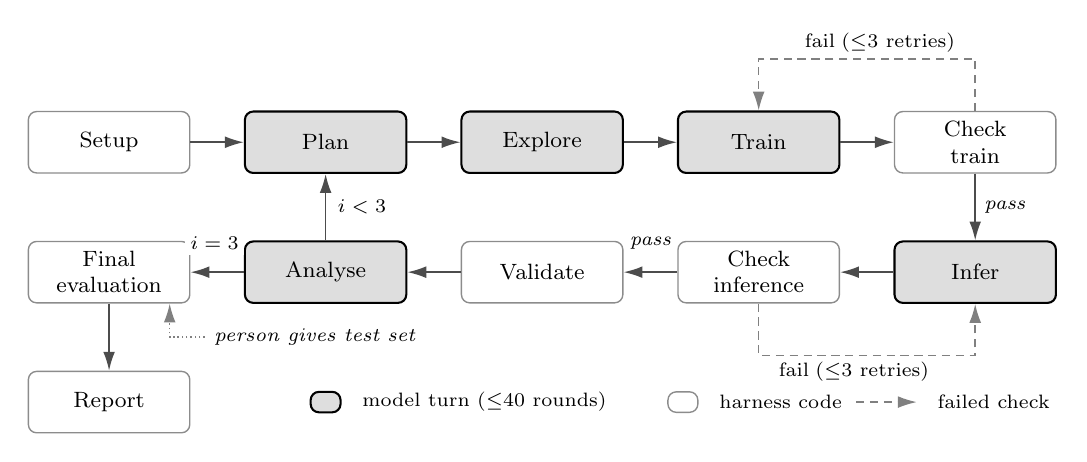
\begin{tikzpicture}[x=2.75cm, y=1.65cm,
    >={Latex[length=2.4mm, width=1.5mm]}, font=\footnotesize,
    every node/.style={align=center},
    % model turns: clearly shaded
    model/.style={draw=black, line width=0.75pt, rounded corners=3pt,
                  fill=black!13, minimum width=2.05cm, minimum height=0.78cm},
    % harness code: outlined only
    code/.style={draw=black!45, line width=0.5pt, rounded corners=3pt,
                 fill=white, minimum width=2.05cm, minimum height=0.78cm},
    edge/.style={->, draw=black!70, line width=0.6pt},
    fail/.style={->, draw=black!50, line width=0.55pt, densely dashed},
    lbl/.style={font=\scriptsize, inner sep=2pt, fill=white}]

  % ── top row (left → right) ──
  \node[code]  (setup)   at (0,0)  {Setup};
  \node[model] (plan)    at (1,0)  {Plan};
  \node[model] (explore) at (2,0)  {Explore};
  \node[model] (train)   at (3,0)  {Train};
  \node[code]  (ctrain)  at (4,0)  {Check\\train};

  % ── bottom row (right → left) ──
  \node[model] (infer)   at (4,-1) {Infer};
  \node[code]  (cinfer)  at (3,-1) {Check\\inference};
  \node[code]  (valid)   at (2,-1) {Validate};
  \node[model] (analyse) at (1,-1) {Analyse};
  \node[code]  (final)   at (0,-1) {Final\\evaluation};
  \node[code]  (report)  at (0,-2) {Report};

  % ── main flow ──
  \draw[edge] (setup)   -- (plan);
  \draw[edge] (plan)    -- (explore);
  \draw[edge] (explore) -- (train);
  \draw[edge] (train)   -- (ctrain);
  \draw[edge] (ctrain)  -- node[lbl, right=1pt] {\itshape pass} (infer);
  \draw[edge] (infer)   -- (cinfer);
  \draw[edge] (cinfer)  -- node[lbl, above=6pt] {\itshape pass} (valid);
  \draw[edge] (valid)   -- (analyse);
  \draw[edge] (analyse) -- node[lbl, right=2pt] {$i < 3$} (plan);
  \draw[edge] (analyse) -- node[lbl, above=6pt, pos=0.55] {$i = 3$} (final);
  % the test set is handed over by the person, after the last iteration
  \node[font=\scriptsize\itshape] (hil) at (0.95,-1.5) {person gives test set};
  \draw[->, draw=black!50, line width=0.55pt, densely dotted] (hil.west) -| ($(final.south)+(0.28,0)$);
  \draw[edge] (final)   -- (report);

  % ── fail loops ──
  \draw[fail] (ctrain.north) -- ++(0,0.4) -|
      node[lbl, above, pos=0.22] {fail\;(${\le}3$ retries)} (train.north);
  \draw[fail] (cinfer.south) -- ++(0,-0.4) -|
      node[lbl, below, pos=0.22] {fail\;(${\le}3$ retries)} (infer.south);

  % ── legend ──
  \node[model, minimum width=0.38cm, minimum height=0.26cm, inner sep=0] (lm) at (1.0,-2) {};
  \node[font=\scriptsize, anchor=west] at (lm.east) {\enspace model turn (${\le}40$ rounds)};
  \node[code,  minimum width=0.38cm, minimum height=0.26cm, inner sep=0] (lc) at (2.65,-2) {};
  \node[font=\scriptsize, anchor=west] at (lc.east) {\enspace harness code};
  \draw[fail] (3.45,-2) -- ++(0.28,0);
  \node[font=\scriptsize, anchor=west] at (3.73,-2) {\enspace failed check};
\end{tikzpicture}

\caption{State-machine condition: the Agentomics-ML procedure.}\label{fig:harness}
\end{subfigure}

\vspace{1.2em}
\begin{subfigure}{\linewidth}\centering
% Skill-condition agent: one state machine state (Model turn) and the skill it loads.
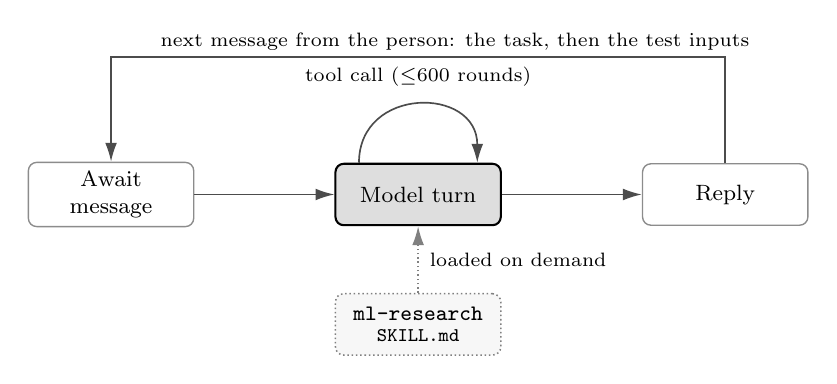
\begin{tikzpicture}[x=2.6cm, y=1.5cm,
    >={Latex[length=2.4mm, width=1.5mm]}, font=\footnotesize,
    every node/.style={align=center},
    model/.style={draw=black, line width=0.75pt, rounded corners=3pt,
                  fill=black!13, minimum width=2.1cm, minimum height=0.78cm},
    code/.style={draw=black!45, line width=0.5pt, rounded corners=3pt,
                 fill=white, minimum width=2.1cm, minimum height=0.78cm},
    doc/.style={draw=black!50, line width=0.55pt, rounded corners=3pt,
                fill=black!3, minimum width=2.1cm, minimum height=0.78cm,
                densely dotted},
    edge/.style={->, draw=black!70, line width=0.6pt},
    lbl/.style={font=\scriptsize, inner sep=2pt, fill=white}]

  \node[code]  (wait)  at (0,0)    {Await\\message};
  \node[model] (turn)  at (1.5,0)  {Model turn};
  \node[code]  (reply) at (3,0)    {Reply};
  \node[doc]   (skill) at (1.5,-1.1)
      {\texttt{ml-research}\\[-2pt]{\scriptsize\texttt{SKILL.md}}};

  % main flow
  \draw[edge] (wait)  -- (turn);
  \draw[edge] (turn)  -- (reply);

  % wrap-around back to Await message
  \draw[edge] (reply.north) -- ++(0,0.9) -|
      node[lbl, above, pos=0.22] {next message from the person: the task, then the test inputs} (wait.north);

  % self-loop for tool calls
  \draw[edge] ($(turn.north west)+(0.12,0)$)
      .. controls +(0,0.65) and +(0,0.65) ..
      node[above=3pt, font=\scriptsize] {tool call (${\le}600$ rounds)}
      ($(turn.north east)+(-0.12,0)$);

  % skill loaded on demand
  \draw[->, draw=black!50, line width=0.55pt, densely dotted]
      (skill.north) -- node[lbl, right=2pt] {loaded on demand} (turn.south);
\end{tikzpicture}

\caption{Skill condition: a general-purpose agent with the \texttt{ml-research} skill.}\label{fig:agent}
\end{subfigure}
\caption{State diagrams of the two conditions. Shaded states are model turns; white states are deterministic code. In
(a), a failed check returns control to the model state that produced the script, at most three times per step; $i$ is
the iteration number. In (b), all control flow inside a turn is decided by the model; the skill is text the model may
load and follow. In both, the person hands over the test set only after the last iteration.}
\label{fig:machines}
\end{figure}

\paragraph{State machine (Agentomics-ML).} The state-machine condition implements the Agentomics-ML procedure on our
agent runtime. It has eleven states (\cref{fig:harness,tab:states}). Five are model
turns, each limited to 40 rounds (a round is one model call and the tool calls it requests). The other six are the
harness's own code: it sets up the data, runs the model's \texttt{train.py} and \texttt{inference.py} on a small split,
checks that predictions have the expected format, scores validation and training data, and keeps the best model so far.
A failed check returns the model to the step that produced the faulty script, up to three times; after that, the
iteration is recorded as failed. Every model turn starts a new conversation. Within an iteration a step is given the
written answers of the steps before it; the planning step of a new iteration is given a history of the finished ones:
each one's plan, its reports on training and inference, its analysis and its validation and training scores. The
files of earlier iterations remain in the workspace for the model to read. After three iterations the harness asks the person for the test set, a
human-in-the-loop step, scores the best model once and writes a report. Three iterations was chosen as a balance between performance and cost.

\begin{table}[tbp]\centering\small
\caption{States of Agentomics-ML (\cref{fig:harness}).}\label{tab:states}
\begin{tabular}{@{}l l p{9.2cm}@{}}\toprule
State & Executed by & Action\\\midrule
Setup & harness & Seeded, stratified 80/20 split; writes a small training subset for checks; installs libraries.\\
Plan & model & Decides what to try in this iteration.\\
Explore & model & Inspects the data and reports findings.\\
Train & model & Writes and runs \texttt{train.py}.\\
Check train & harness & Re-runs \texttt{train.py} on the small subset.\\
Infer & model & Writes \texttt{inference.py}.\\
Check inference & harness & Runs \texttt{inference.py} on the small subset and checks the predictions' format.\\
Validate & harness & Scores validation and training data; copies the best iteration so far to \texttt{best/}.\\
Analyse & model & Reviews the iteration and proposes changes for the next.\\
Final evaluation & harness & Asks the person for the test set (human in the loop) and scores the best model once.\\
Report & harness & Writes \texttt{metrics.json} and \texttt{report.md}.\\
\bottomrule\end{tabular}
\end{table}

\paragraph{Skill.} The skill condition uses a general-purpose agent with a single state (\cref{fig:agent}): it waits for
a message, takes one turn of up to 600 rounds, and replies. 600 rounds equals the harness's total budget (40 rounds,
five model steps, three iterations); cost and time were not fixed, and are outcomes. The agent's system prompt names its tools and tells it to load a skill when one
covers the task; apart from the skill's one-line description it contains nothing about machine learning. The skill, \texttt{ml-research}, describes the same
procedure as the harness (\cref{app:repro}): a seeded split, a check run the same way the test will be, three
iterations with the best chosen on validation, and a test step. It ships scripts for the split, the check and the
scoring, but the agent decides whether to run them; nothing outside the agent enforces the procedure. The test set
enters through a human-in-the-loop step here too: when the agent reports that its iterations are done, the person
gives it the test inputs, without labels, and it predicts once with the model it selected. In our runs a script
answered these requests in the person's place, through the runtime's AG-UI interface \citep{agui2025}, the protocol by which an agent asks its user for
input, and in the same way for every run of both conditions. The agent keeps one
conversation for the whole task, so each iteration is carried out with everything from the earlier ones in view.
The runtime would prune older tool outputs and summarise earlier turns if a prompt filled 80\% of the model's context
window; no original skill run came near that, the largest prompt being about 105,000 tokens.

\subsection{Models and reasoning effort}\label{sec:models}

Nine models were used, all through OpenRouter: Claude Fable 5.2, Claude Opus 5.5, GPT-6.2 Astra, Gemini 4 Hydrogen,
Claude Sonnet 5.5, Qwen 3.5 122B-A10B, Claude Haiku 4.5, DeepSeek V4.1 Flash and GPT-4.1. We group them into
\emph{top-of-line} models (Fable 5.2, Opus 5.5, Astra, Hydrogen), each being the highest-capability offering from its
provider's current line-up at the time of the experiment, and \emph{mid-range} models (Sonnet 5.5, Qwen 3.5 122B-A10B,
Haiku 4.5, DeepSeek V4.1 Flash, and GPT-4.1, an earlier-generation model included because the published Agentomics-ML
results use it); we use this grouping in the analysis. Each ran under both conditions with
the reasoning-effort setting at \texttt{none} and at \texttt{high} (the largest thinking budget), giving
$9 \times 2 \times 2 = 36$ runs. Our runtime sends \texttt{none} to OpenRouter as a request for minimal effort, and
providers map the field to their own token budgets, so \texttt{none} did not switch reasoning off: only Astra and
GPT-4.1 produced no reasoning tokens with it (\cref{tab:runs}). GPT-4.1 does
not reason: it produced no reasoning tokens at either setting, so its two runs per method are in effect repeats.

\subsection{Repeated runs}\label{sec:repeats}

Nine of the 36 runs reported here are repeats, made on 20--21 November 2026 with a second implementation of the two
conditions: all four GPT-4.1 runs, both Astra runs with reasoning \texttt{high}, and the state-machine runs of Opus,
Gemini and Sonnet with reasoning \texttt{none}. They were chosen after their test scores were known: the GPT-4.1
state-machine runs had both ended after two iterations, the state-machine runs of Opus and Sonnet had a validation
score far above their test score, that of Gemini had been completed by hand, and Astra's skill score with reasoning
\texttt{high}, below its state-machine score, was unexpected. A repeat replaces the original run in every table and
figure; \cref{tab:repeats} gives both scores, and repeats are marked in \cref{tab:matrix,tab:pairs,tab:runs}.

\begin{table}[tbp]\centering\small
\caption{The nine repeated configurations: test AU-PRC of the original run and of the repeat that replaces it, with the
number of iterations that produced a scored model (It.). $\Delta$: repeat minus original.}
\label{tab:repeats}
\RepeatTable
\end{table}

The second implementation runs Agentomics-ML 1.2.0 from its published container image, with the reasoning effort set
on every request and a failing script returned to its step three times, not its default five, its tool for fetching papers switched off, and a second
general-purpose agent for the skill. It differs from the original in its steps (Agentomics-ML 1.2.0 has eight model
steps per iteration), its round limits (100 per step and 1,500 for the skill agent), its split (made once by the
skill's setup script for both conditions), its prompts (Agentomics-ML used its default task prompt) and its time
accounting (elapsed time to the end of the last iteration). It sends the reasoning setting as given; OpenRouter refused
\texttt{none} for Opus, Gemini, Sonnet and Astra, so the state-machine repeats of Opus and Gemini ran at
\texttt{minimal}, the value their originals had been sent, and that of Sonnet at \texttt{low}, and Astra's runs with
reasoning \texttt{none} remain the originals.

\subsection{Evaluation}\label{sec:evaluation}

The primary outcome is test AU-PRC (average precision), computed from each run's predicted class probabilities on the held-out test set. We also report test accuracy from the run's own hard label predictions and, where available, training accuracy. The test set was never given to an agent while it was training; once all runs had finished, we collected each run's prediction file and scored it in a single controlled step, outside the agent environment, to ensure consistent evaluation conditions across all runs.

To study iterations, we re-ran each iteration's saved model on the test inputs in a single controlled environment,
pinned to the library versions the original runs used. As a consistency check we also recomputed each run's validation AU-PRC; every value
matched the run's own record to four decimal places. The model a run would have submitted after $k$ iterations is the
one with the best validation score among its first $k$, which is the selection rule both conditions use.

\subsection{Cost and time}\label{sec:accounting}

Cost is the amount OpenRouter billed for each call, summed per run. Time is training time: the time the model spent
answering plus the time the run's commands took (feature building, training, and the checks and scoring of each
iteration, whether the agent or the harness ran them), up to the end of the last iteration. Time in which neither the
model nor a command was working is not counted, and neither is the final evaluation on the test set.

\section{Results}\label{sec:results}

\subsection{Test performance}

The results divide by model tier. Top-of-line models score \FlagScoreMin--\FlagScoreMax{} across all
conditions and both methods: for these models the method makes little practical difference. Mid-range models
vary more (\SmallScoreMin--\SmallScoreMax); here the state machine wins more often. \Cref{tab:matrix} gives the score of every run and \cref{fig:scores}
plots them; \cref{tab:pairs} compares the two methods pair by pair with 95\% confidence intervals. Cost and time are
in \cref{sec:cost}.

\begin{table}[tbp]\centering\small
\caption{Test AU-PRC (average precision) by model, method and reasoning effort. Each model's best run is marked in
bold; the best overall is marked bold and underlined. $^{\dagger}$: a repeated run (\cref{sec:repeats}).
$^{\ddagger}$: test predictions produced by hand from the run's selected model (\cref{sec:limitations}).}
\label{tab:matrix}
\MatrixTable
\end{table}

\begin{figure}[tbp]\centering
% Every run's test AU-PRC, one row per model (series from generated.tex).
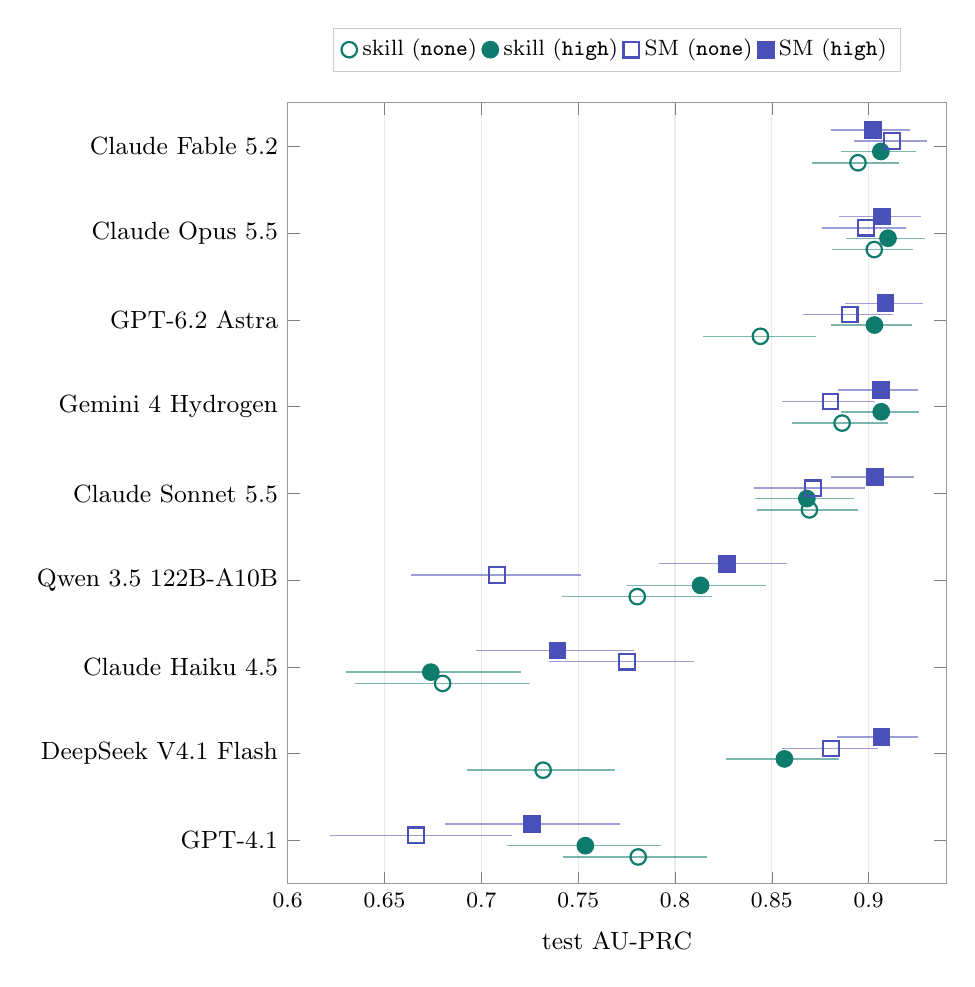
\begin{tikzpicture}
\begin{axis}[width=0.82\linewidth, height=11.5cm, xmin=0.60, xmax=0.94, ymin=0.5, ymax=9.5,
  dotrows, yticklabel style={font=\small}, xlabel={test AU-PRC},
  xmajorgrids, grid style={black!8}, axis line style={black!40},
  xlabel style={yshift=-2pt},
  legend style={font=\footnotesize, at={(0.5,1.04)}, anchor=south, draw=black!20, fill=white, legend columns=4},
  legend cell align=left,
  every legend image/.append style={mark size=2.5pt},
  every axis plot/.append style={only marks, mark size=2.8pt}]
\DotPlots
\legend{{skill (\texttt{none})},{skill (\texttt{high})},{SM (\texttt{none})},{SM (\texttt{high})}}
\end{axis}
\end{tikzpicture}

\caption{Test AU-PRC of every run. Circles: skill; squares: state machine (Agentomics-ML). Filled: reasoning \texttt{high}; open: reasoning \texttt{none}. The bar through each marker is the run's 95\% bootstrap
interval (test-set sampling only).}
\label{fig:scores}
\end{figure}


\begin{table}[tbp]\centering\small
\caption{Paired comparison on the test set. SM: state machine (Agentomics-ML). $\Delta$: SM minus skill. 95\% CI:
percentile interval over 2,000 paired bootstrap resamples; $\Delta$ in bold where the interval excludes zero.
The interval reflects test-set sampling only, not run-to-run variation (\cref{sec:limitations}). $^{\dagger}$,
$^{\ddagger}$: as in \cref{tab:matrix}.}
\label{tab:pairs}
\PairTable\\[0.4em]
\PairTableNote
\end{table}

\paragraph{Score uncertainty.} Each run is evaluated on the same 1,018 held-out test examples, and those specific examples introduce sampling variation: a model that scores 0.80 on this test set might score differently on a different draw from the same distribution. To quantify this, we resampled the test set 2,000 times with replacement and recomputed AU-PRC each time; the central 95\% of that distribution gives a confidence interval for the run's score. For a typical run, this interval extends roughly \CIHalfMed{} in each direction, so a difference of that size or smaller between two rows of \cref{tab:matrix} may reflect the particular test examples rather than a genuine performance gap.

The paired comparison in \cref{tab:pairs} is more reliable for judging the two methods head to head: because both methods are scored on the same test examples, most of that sampling noise cancels in the difference. Across the \WilcoxonN{} model-and-reasoning pairs, the state machine is clearly better in \PairsSm{}, the skill in \PairsSkill{}, and \PairsTie{} are indistinguishable. Taken together, neither method has a clear overall edge (Wilcoxon signed-rank test, $p=\WilcoxonP$, median difference \MedianDiff{}): the state machine's wins on three mid-range models are offset by ties on top-of-line models and by the pairs the skill wins. With the original runs in place of the nine repeats the counts are \OrigPairsSm{}, \OrigPairsSkill{} and \OrigPairsTie{} ($p=\OrigWilcoxonP$; \cref{sec:repeats}).

\paragraph{Top-of-line models perform alike under both methods.} With reasoning
\texttt{high}, all \FlagHighTies{} top-of-line pairs are ties, the largest difference being \FlagHighMax. With reasoning
\texttt{none}, the state machine is ahead for Fable and Astra; the
skill catches up once the model reasons.

\paragraph{Mid-range models gain from the state machine, with exceptions.} Among the other five models the state
machine is clearly better in \SmallSm{} of \SmallPairs{} pairs (Haiku and DeepSeek at both settings, and Sonnet with reasoning \texttt{high}) and the
skill in \SmallSkill{}: Qwen 3.5 122B and GPT-4.1, both with reasoning \texttt{none}. The
remaining three pairs, Sonnet with reasoning \texttt{none} and Qwen and GPT-4.1 with reasoning \texttt{high}, are ties
(\cref{tab:pairs}; GPT-4.1 is discussed in \cref{sec:agentomics}).

Higher reasoning effort improved test AU-PRC in \HighWins{} of the \HighPairs{} model--method pairs, which is not distinguishable
from chance. The best single run was \BestCell, at \BestScore.

\subsection{Iterations}\label{sec:iterations}

\Cref{fig:itermeans} shows the mean test AU-PRC of the model a run would have submitted after one, two and three
iterations, for each tier, method and reasoning setting. \Cref{fig:iterations} shows every model separately, and \cref{tab:iterations} in \cref{app:tables} gives the
numbers, the iteration each run submitted and the iteration whose model scored best on test.

\begin{figure}[tbp]\centering
% Mean test AU-PRC after 1, 2 and 3 iterations, by tier, method and reasoning effort (series from generated.tex).
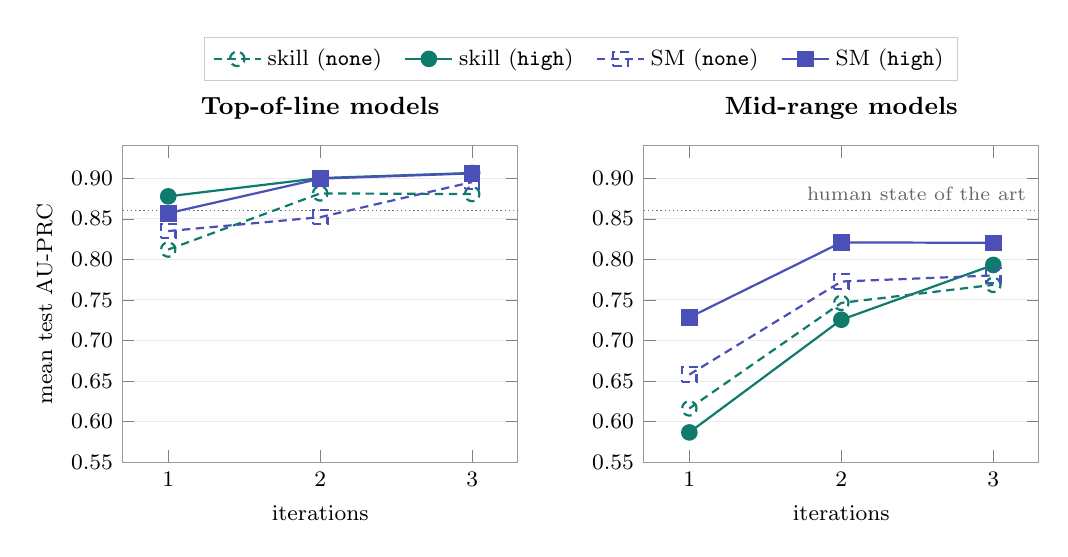
\begin{tikzpicture}
\begin{groupplot}[group style={group size=2 by 1, horizontal sep=1.6cm},
  width=6.6cm, height=5.6cm, xmin=0.7, xmax=3.3, xtick={1,2,3}, ymin=0.55, ymax=0.94,
  ytick={0.55,0.60,0.65,0.70,0.75,0.80,0.85,0.90},
  ytick scale label code/.code={}, scaled y ticks=false,
  yticklabel style={/pgf/number format/fixed, /pgf/number format/fixed zerofill, /pgf/number format/precision=2},
  title style={font=\small\bfseries}, axis line style={black!40}, label style={font=\footnotesize},
  ymajorgrids, grid style={black!8},
  every axis plot/.append style={mark size=2.6pt, line width=1.1pt}]
\IterMeanPlots
\end{groupplot}
\node[anchor=south] at ($(group c1r1.north)!0.5!(group c2r1.north)+(0,0.7cm)$) {\pgfplotslegendfromname{itermeanlegend}};
\end{tikzpicture}

\caption{Mean test AU-PRC of the model a run would have submitted after 1, 2 and 3 iterations, by model tier. Circles:
skill; squares: state machine (Agentomics-ML). Solid lines and filled markers: reasoning \texttt{high}; dashed lines
and open markers: reasoning \texttt{none}. Both panels share one y-axis; the dotted line is the human state of the art (0.860). A run with no working model yet is left out
of that point's mean, and a run with fewer iterations keeps what it ended with. \Cref{fig:iterations} shows every model separately.}
\label{fig:itermeans}
\end{figure}

\begin{figure}[tbp]\centering
% Test AU-PRC of the model each run would have submitted after 1, 2 and 3 iterations (series from generated.tex).
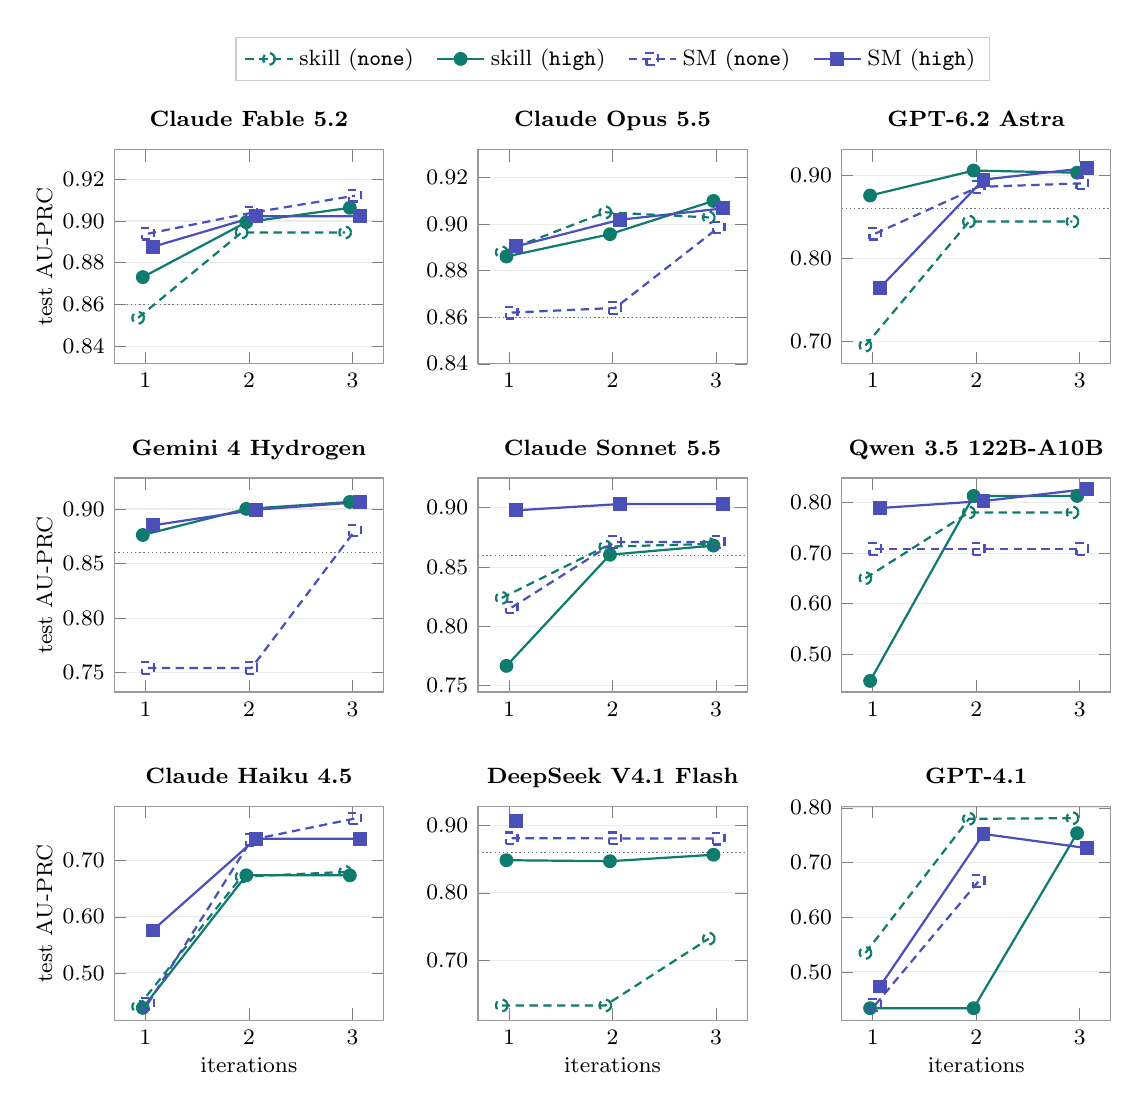
\begin{tikzpicture}
\begin{groupplot}[group style={group size=3 by 3, horizontal sep=1.2cm, vertical sep=1.45cm},
  width=5.0cm, height=4.3cm, xmin=0.7, xmax=3.3, xtick={1,2,3},
  enlarge y limits={abs=0.022},
  ytick scale label code/.code={}, scaled y ticks=false,
  yticklabel style={/pgf/number format/fixed, /pgf/number format/fixed zerofill, /pgf/number format/precision=2},
  title style={font=\footnotesize\bfseries, yshift=-3pt, text height=1.6ex, text depth=0.4ex}, axis line style={black!40},
  label style={font=\footnotesize}, xlabel style={yshift=2pt}, ylabel style={yshift=-3pt},
  ymajorgrids, grid style={black!8},
  every axis plot/.append style={mark size=2.1pt, line width=0.9pt}]
\IterPlots
\end{groupplot}
\node[anchor=south] at ($(group c2r1.north)+(0,0.75cm)$) {\pgfplotslegendfromname{iterlegend}};
\end{tikzpicture}

\caption{Test AU-PRC of the model each run would have submitted after 1, 2 and 3 iterations, one panel per model.
Circles: skill; squares: state machine (Agentomics-ML). Solid lines and filled markers: reasoning \texttt{high};
dashed lines and open markers: reasoning \texttt{none}. Dotted line: the human state of the art (0.860), where a
panel's range reaches it. Each panel has its own y-axis, so slopes compare within a panel, not across panels;
points are nudged sideways so that equal scores stay apart.}
\label{fig:iterations}
\end{figure}

Most of the gain arrives by the second iteration. Top-of-line models mostly start at 0.85--0.89 and add 0.01--0.04 afterwards; the exceptions are Astra and Gemini with
reasoning \texttt{none}, which start between 0.69 and 0.83, and Astra under the state machine with reasoning \texttt{high} (0.76). Mid-range models make their largest step at iteration 2
(Haiku rises from 0.44--0.58 to 0.67--0.74). Later iterations
can be by far the most expensive: DeepSeek under the state machine with reasoning \texttt{none} had 0.881 after seven
minutes, and its second and third iterations took a further 140 minutes without improving on it.

\paragraph{Single shot.} \Cref{tab:single} compares the two methods after the first iteration only, as if each run had
been given one attempt, pair by pair and with the same paired bootstrap as \cref{tab:pairs}. Seventeen of the eighteen pairs can be compared this way; the eighteenth is Gemini with reasoning \texttt{none},
whose skill run had no working model after its first iteration. Among the seventeen the state machine is the stronger
single shot: it is clearly ahead in \FirstCiSm{}, the skill in \FirstCiSkill{}, and \FirstCiTie{} are ties (Wilcoxon
signed-rank test, $p\FirstWilcoxonP$, median difference \FirstMedianDiff). The advantage is clearest among mid-range models:
\FirstMidCiSm{} of the \FirstMidCiPairs{} mid-range pairs, against \FirstFlagCiSm{} of the \FirstFlagCiPairs{}
top-of-line pairs. On average the state machine's first model scores \FirstSmMean{} and the skill's \FirstSkillMean{}.

The skill catches up once it is allowed to iterate. After one iteration the state machine leads by \FirstGap{} on
average; by the end its lead is \FinalGap. Mid-range models have the most to gain from iterating: their later
iterations add \FirstSmallGain{} on average, against \FirstFlagGain{} for top-of-line models. For many runs a single
attempt is already enough to be competitive: \FirstAboveSota{} of the \FirstRuns{} first models beat the human state
of the art.

\begin{table}[tbp]\centering\small
\caption{Single-shot comparison: test AU-PRC of the model each run had after its first iteration. SM: state machine
(Agentomics-ML). $\Delta$: SM minus skill, with a 95\% paired bootstrap interval as in \cref{tab:pairs}; bold where the
interval excludes zero. N/A: no working model after the first iteration. $^{\dagger}$, $^{\ddagger}$: as in
\cref{tab:matrix}.}
\label{tab:single}
\FirstPairTable
\end{table}

\paragraph{How many iterations.} \Cref{tab:budget} shows what each method has after one, two and three iterations,
and what share of its total cost and training time it has spent by then. Two iterations capture most of the result:
stopping there lowers the mean score by \TwoLoss{} and uses \TwoCostShare\% of the cost and \TwoTimeShare\% of the
training time. \TwoWithin{} of the \TwoRuns{} runs with a model after two iterations are already within 0.005 of their
final score.

\begin{table}[tbp]\centering\small
\caption{Iteration budget: the mean test AU-PRC each method has after one, two and three iterations (the model a run
would have submitted at that point), with the share of the method's total cost and training time spent by then. A run
with fewer iterations keeps what it ended with.}
\label{tab:budget}
\BudgetTable
\end{table}

\paragraph{A run does not always submit its best model.} Each run submits the iteration that scored highest on its
own validation data, since it never sees the test set. That is usually, but not always, the iteration that scores
highest on test: the two agree in \PickedBest{} of the \ScoredRuns{} runs. The clearest miss is GPT-4.1 under the state
machine with reasoning \texttt{high}. Its second iteration scored 0.752 on test, but its third scored slightly higher
on validation (0.721 against 0.705) and was submitted instead, at 0.726.
In the other runs where the two disagree, the cost is at most 0.020.

\subsection{Comparison with Agentomics-ML}\label{sec:agentomics}

\Cref{tab:agentomics} sets our GPT-4.1 runs beside those published for Agentomics-ML \citep{martinek2025agentomics} on
the same dataset and the same train/test split, with average precision, the metric used here. We make this comparison
for GPT-4.1 only, the model the published results use: the other models here are newer, and setting their scores
against the published ones would measure the models, not the method.

\begin{table}[tbp]\centering\small
\caption{Test AU-PRC (average precision) of GPT-4.1 on AGO2 CLASH. Agentomics-ML as reported by
\citet{martinek2025agentomics}, arXiv v1, over five runs per configuration. This study: two runs per method.}
\label{tab:agentomics}
\begin{tabular}{@{}l l r r@{}}\toprule
\textbf{Method} & \textbf{Model} & \textbf{Mean} & \textbf{Best}\\\midrule
Agentomics-ML, no feedback & GPT-4.1 & 0.698 & 0.724\\
Agentomics-ML & GPT-4.1 & 0.726 & 0.778\\\midrule
State machine (this study) & GPT-4.1, 2 runs & \GptSmMean & \GptSmBest\\
Skill (this study) & GPT-4.1, 2 runs & \GptSkillMean & \GptSkillBest\\
\bottomrule\end{tabular}
\end{table}

\paragraph{GPT-4.1 under both methods.} GPT-4.1 is the one model both studies share; all four of its runs here are
repeats made with Agentomics-ML 1.2.0 and the second skill agent (\cref{sec:repeats}). Under the state machine it scored
\GptSmNone{} and \GptSmHigh{} (two runs that are in effect repeats, \cref{sec:models}); in the first, the third iteration
failed its checks and the second was submitted. \GptSmHigh{} equals the mean Agentomics-ML reports for GPT-4.1 (means
of 0.698 and 0.726, best run 0.778) and \GptSmNone{} falls just below it, so our runs are broadly consistent with the
published result on the one model the two share.

Under the skill it scored \GptSkillNone{} and \GptSkillHigh{}, completing all three iterations in both runs for
\$5.92 and \$0.33, against \$1.50 and \$2.10 with the state machine. The skill is ahead in both pairs; the interval
of the pair at reasoning \texttt{high} includes zero (\cref{tab:pairs}). The oldest model here therefore did not need
the harness on this task: it followed the written procedure to the end and scored at least as well as with enforced
steps.

\subsection{Cost and time}\label{sec:cost}

The skill used \SkillCost{} and \SkillTime{} over its eighteen runs, \CostRatio{} of the cost and \TimeRatio{} of the
time of the state machine (\SmCost{} and \SmTime). The difference comes mostly from the number of model calls
(\SkillCalls{} against \SmCalls): the state machine starts a fresh model turn at every step, each with its own context,
whereas the agent works through the task in one turn. One state-machine record, Fable with reasoning \texttt{high},
sums two runs and accounts for \FableSmHighCost{} of that total (\cref{sec:limitations}). \Cref{fig:time} shows the cost and training time of every run and how the time divides across iterations;
\cref{tab:cost,tab:time} give the numbers.

\begin{table}[tbp]\centering\small
\caption{Cost per run in USD, as billed by OpenRouter. Each model's cheapest run is marked in bold; the cheapest overall
is marked bold and underlined.}
\label{tab:cost}
\CostTable
\end{table}

\begin{table}[tbp]\centering\small
\caption{Training time per run in minutes: model time plus code time up to the end of the last iteration (\cref{sec:accounting}). Each model's fastest run is marked in
bold; the fastest overall is marked bold and underlined.}
\label{tab:time}
\TimeTable
\end{table}

\begin{figure}[tbp]\centering
% Cost and training time per run on log axes, and each run's split of time across its iterations (series from generated.tex).
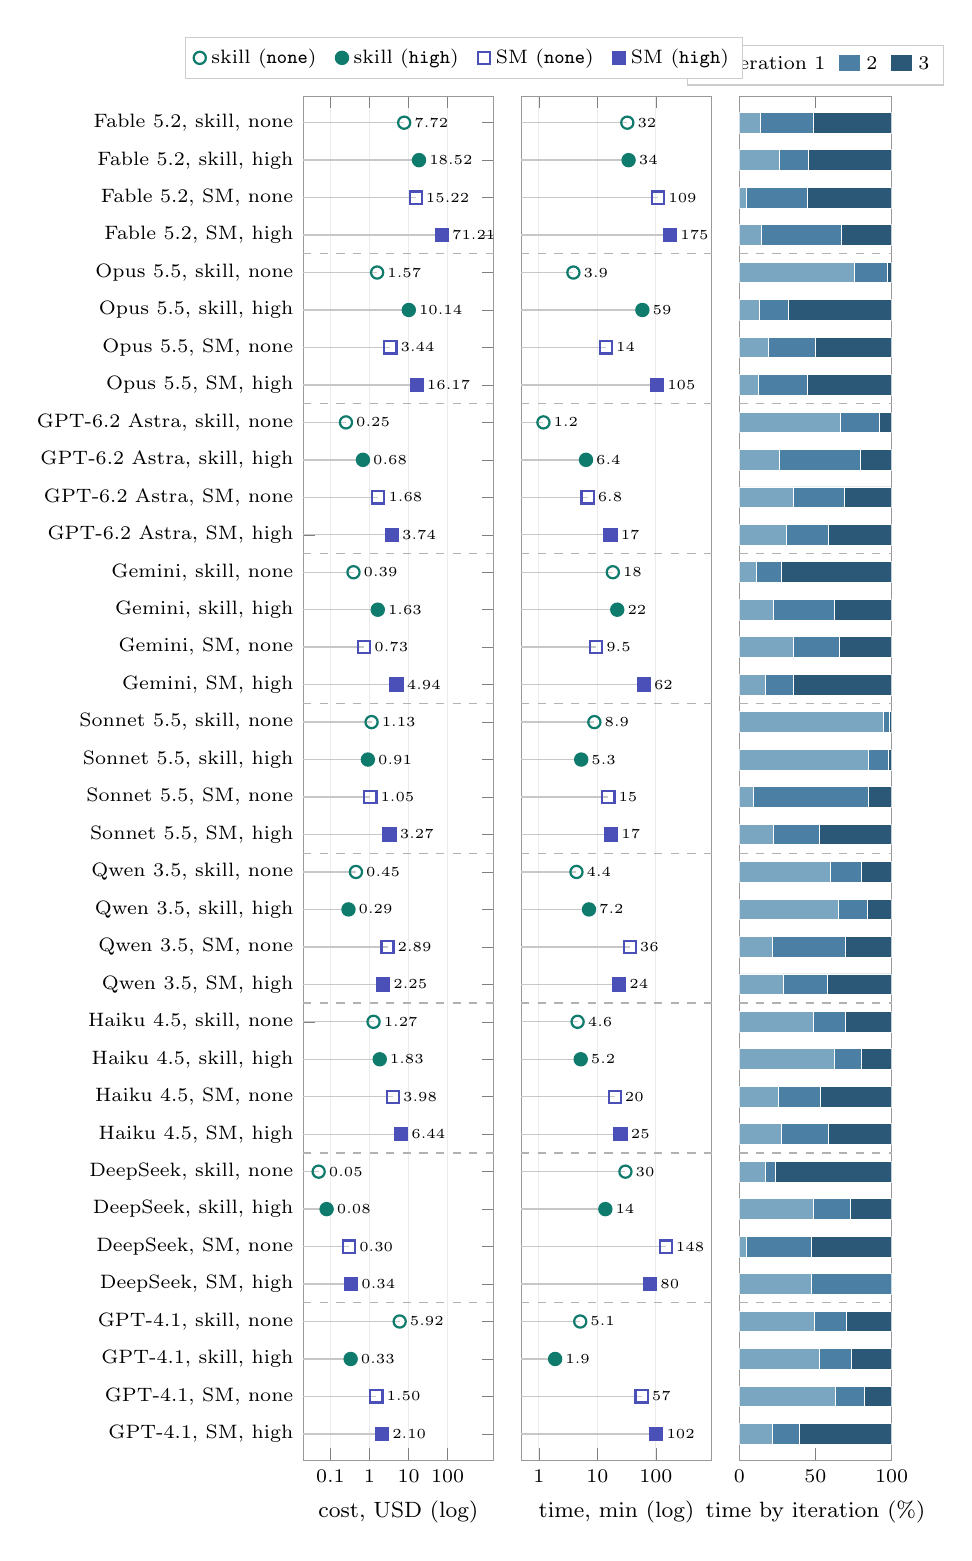
\begin{tikzpicture}
\pgfplotsset{runrows/.style={height=18.9cm, ymin=-0.7, ymax=35.7, axis line style={black!40},
  label style={font=\footnotesize}, tick label style={font=\scriptsize},
  extra y ticks={3.5,7.5,11.5,15.5,19.5,23.5,27.5,31.5}, extra y tick labels={,,,,,,,},
  extra y tick style={grid=major, grid style={draw=black!30, line width=0.5pt, dashed}, tick style={draw=none}}}}
\begin{axis}[name=cost, runrows, xmode=log, log basis x=10, width=0.33\linewidth, xmin=0.02, xmax=1500,
  xtick={0.1,1,10,100}, xticklabels={0.1,1,10,100}, timerows, yticklabel style={font=\scriptsize},
  xlabel={cost, USD (log)}, xmajorgrids, grid style={black!8}, every axis plot/.append style={mark size=2.2pt},
  legend to name=runlegend, legend columns=4, legend style={font=\scriptsize, draw=black!20, /tikz/every even column/.append style={column sep=0.5em}}]
\CostTotalPlots
\legend{{skill (\texttt{none})},{skill (\texttt{high})},{SM (\texttt{none})},{SM (\texttt{high})}}
\end{axis}
\begin{axis}[name=totals, at={(cost.east)}, anchor=west, xshift=0.35cm, runrows, xmode=log, log basis x=10, width=0.33\linewidth,
  xmin=0.5, xmax=900, xtick={1,10,100}, xticklabels={1,10,100}, ytick={0,...,35}, yticklabels={}, ytick style={draw=none},
  xlabel={time, min (log)}, xmajorgrids, grid style={black!8}, every axis plot/.append style={mark size=2.2pt}]
\TimeTotalPlots
\end{axis}
\begin{axis}[name=share, at={(totals.east)}, anchor=west, xshift=0.35cm, runrows, xbar stacked, bar width=7.5pt, width=0.29\linewidth,
  xmin=0, xmax=100, xtick={0,50,100}, ytick={0,...,35}, yticklabels={}, ytick style={draw=none},
  xlabel={time by iteration (\%)},
  legend style={font=\scriptsize, at={(0.5,1.008)}, anchor=south, legend columns=3, draw=black!20, /tikz/every even column/.append style={column sep=0.25em}}]
\TimeSharePlots
\legend{iteration 1, 2, 3}
\end{axis}
\node[anchor=south] at ($(cost.north)!0.5!(totals.north)+(-0.55cm,0.1cm)$) {\pgfplotslegendfromname{runlegend}};
\end{tikzpicture}

\caption{Cost and training time of every run. Runs group by model, four per model (skill or state machine, reasoning
\texttt{none} or \texttt{high}). Left: cost in USD; middle: training time in minutes; both on log scales, with the
value beside each marker (circles: skill, squares: state machine, filled: reasoning \texttt{high}). Right: how the
training time divides across iterations 1, 2 and 3. The state machine records the iteration it is in; for a skill run
an iteration is taken to end when the agent first writes into the next iteration's folder, so its split is
approximate. DeepSeek's state-machine run with reasoning \texttt{high} stopped during its second iteration, and Gemini's skill run with
reasoning \texttt{none} took five, the last three drawn together.}
\label{fig:time}
\end{figure}

\section{Discussion}\label{sec:discussion}

For top-of-line models with reasoning enabled, written guidance was enough: with reasoning \texttt{high}, the skill and
Agentomics-ML are indistinguishable on the test set for all four, and the skill costs a fraction as much. With
reasoning \texttt{none}, Agentomics-ML's fixed steps still help two of the four (Fable and Astra),
suggesting that its structure partly substitutes for the model planning its own work.

For three of the five mid-range models Agentomics-ML helps clearly: Haiku and DeepSeek score higher with it
at both reasoning settings, and Sonnet with reasoning \texttt{high}. The simplest explanation, that agents skip the skill's checks, does not hold: sixteen of the eighteen
skill runs ran the check script on every iteration and passed it (\cref{sec:limitations}). What differs is who
drives the procedure. Agentomics-ML gives each stage its own model turn and sends a script that fails back to the
step that wrote it; under the skill one model turn carries the whole task. The single-shot comparison
(\cref{tab:single}) points the same way: the state machine's advantage is largest on the first iteration, before the
agent has had a chance to correct its own course. What each method carries from one iteration to the next may explain
why the skill then catches up: the skill's agent keeps its whole conversation, while each state-machine step starts
afresh from a written summary of the earlier iterations (\cref{sec:conditions}). We did not test this directly.

Qwen 3.5 122B and GPT-4.1 are the exceptions, each in one of its two pairs. Qwen with reasoning \texttt{none} scored higher
with the skill; its state-machine run made no validation progress after its first iteration. GPT-4.1 scored
higher with the skill at both settings, completing three iterations where one of its state-machine runs failed the third; with
one run per setting the gap should not be over-read.

\paragraph{Reasoning and structure.} A state machine can be read as reasoning done in advance: the order of work and
the points at which to check it are decided before the model starts. If so, a model's own reasoning should matter more
under the skill, where that planning is left to it. The data do not settle it. With reasoning
\texttt{high} the skill's mean score rises by \SkillReasonGain{} (from \SkillNoneMean{} to \SkillHighMean), the state
machine's by \SmReasonGain{} (from \SmNoneMean{} to \SmHighMean); reasoning raised the score for \SkillHighWins{} of the 9 models
under the skill and \SmHighWins{} of the 9 under the state machine. The single-shot comparison shows the same pattern
more sharply: on a first attempt, before any feedback, the state machine's structure is worth the most.

The iteration analysis has a practical consequence: a two-iteration budget would have captured most of the
performance for about half the training time (\cref{tab:budget}).

\paragraph{What enforced structure buys.} A recurring question about harness-based agents is whether their structural
guarantees are worth the added complexity compared to a well-written skill or prompt. This experiment offers three observations
on that question. First, enforced structure matters for mid-range models: Sonnet, Haiku and DeepSeek all score
higher with Agentomics-ML, although the skill runs ran the same checks themselves. Second, no run could have seen the test labels while it was training, under either method. The skill makes the
test set a hand-over by the person: the agent finishes its iterations, reports, and only then is given the test
inputs, without labels, to predict on once. The state machine does the same in code: inputs and labels arrive after
the last iteration, for the harness's own final scoring step, when no model step remains; none of the tool calls those
runs made refers to the test upload. Both designs keep the test set out of reach by releasing it late;
the harness enforces the moment, and the skill leaves it to the person. Third, all reported scores were computed from the prediction files the runs wrote, not from anything the model
reported, so metric correctness is independently verified in both conditions. What the experiment does not address is whether
Agentomics-ML's step-wise context management helps or hurts; a direct comparison of full-context and step-wise
execution is a natural next step.

\paragraph{Cost.} The cost gap between the two conditions is large enough to matter in practice. The skill's eighteen
runs cost \SkillCost{} in total, Agentomics-ML's \SmCost{}. Much of the difference is structural: Agentomics-ML starts
a fresh model turn for each of its five model states per iteration, each carrying its own context, while the agent
works through the full task in a single turn. Within each condition, model tier is the dominant cost driver: top-of-line
models averaged \FlagSkillAvgCost{} per skill run and \FlagSmAvgCost{} per Agentomics-ML run, while mid-range models
averaged \SmallSkillAvgCost{} and \SmallSmAvgCost{} respectively. Fable 5.2 with reasoning \texttt{high} stands out at \FableSkillHighCost{} (skill) and \FableSmHighCost{}
(Agentomics-ML, over the two runs its record sums), driven by its large reasoning-token budget; DeepSeek V4.1 Flash, at the other extreme,
averaged under \$0.25 per run. For top-of-line models with reasoning enabled, where test performance is equivalent, the
skill is the more resource-efficient choice. For mid-range models, where Agentomics-ML scores higher, the extra cost
buys the enforced structure. Anyone choosing a configuration should weigh score and cost together.

\section{Limitations}\label{sec:limitations}

\paragraph{One run per configuration.} Each model, method and reasoning setting was run once. The bootstrap intervals
in \cref{tab:pairs} capture the uncertainty of scoring on 1,018 test pairs, not the variation between repeated runs of
the same configuration, which is likely larger: across Agentomics-ML's five GPT-4.1 runs on this dataset the reported
spread is 0.033 \citep[Table 5, given there as the variance between runs]{martinek2025agentomics}. Our own repeats point the same way: for the nine configurations run twice, the two runs differed by a
median of \RepeatMedianDiff{} and by up to \RepeatMaxDiff{} (\cref{tab:repeats}). Differences of a few hundredths between single runs should therefore
be read as directions, and the conclusions rest on patterns that hold across several models rather than on any one pair.


\paragraph{Adherence to the skill.} Nothing enforces the skill's procedure, so we checked every skill run's commands
against it. All eighteen runs ran the skill's setup script, and every recorded score was written by the skill's
scripts; no run wrote the record itself. Sixteen runs ran the check script on each of their three planned iterations
and passed it. The other two are DeepSeek with reasoning \texttt{high}, whose first iteration never passed the check
(its second and third did), and Gemini with reasoning \texttt{none}, which needed five iterations before one passed.
Seventeen runs stopped at the three planned iterations. After the test inputs arrived, no run trained again or changed
its selected model; two copied into the selected model's folder a helper module that its inference script imports.
For the three repeated skill runs no command log was kept, and we checked their workspaces instead.

\paragraph{Test labels in the workspace.} In the state-machine condition the test upload contained its labels file
alongside the inputs, because the harness's final evaluation step scores the model itself. It was uploaded only after a
run's last iteration, when its model had been selected, and the state machine has no model step after that point. No
tool call in any run refers to the labels file. Skill runs received the test inputs only, and none trained again or
changed its selected model once they arrived. In the repeated state-machine runs the test split was not in the model's container during the
iterations. All reported test scores were computed independently.

\paragraph{Interrupted runs.} State-machine runs are long, up to three hours, and they run the agent's training code in
the same container as the agent runtime, under a fixed memory limit. When a training job exceeded that limit the
container was stopped, and because a state-machine run carries out all three iterations in one uninterrupted turn, it
could not continue from where it had stopped. This happened several times, always in state-machine runs with long
training jobs, and is a property of our execution environment, not of either method. Interrupted runs were repeated.
Where a repeat was interrupted as well, the run is reported with the iterations it completed: DeepSeek under the state
machine with reasoning \texttt{high} has one, and Claude Fable 5.2 under the state machine with reasoning
\texttt{high} has two, to which the first iteration of a second run of that configuration was added; that record's
cost, calls and time are those of both runs. No skill run lost an iteration this way; their training jobs
were shorter. Since every reported score is computed from the prediction files a run wrote (\cref{sec:evaluation}), an
interruption after a model was trained does not change how that model is scored.

\paragraph{Runs completed by hand.} In \HandCount{} of the 27 original runs (\HandSm{} state machine, one skill) the run
ended before it had predicted on the test set, and we ran the selected iteration's own inference script on the test
inputs ourselves; they are marked in \cref{tab:matrix,tab:pairs,tab:single,tab:runs}. In three the final step failed
because the selected model's script imported a module that had not been copied with it, in three the run stopped while
waiting for the test set, one failed on a provider error after its third iteration had been scored, two were stopped
during an iteration, and one skill run never reached its test step. The model, its selection on validation and the
inference script are the run's own. In \HandSmAhead{} of the \PairsSm{} pairs in which the state machine is clearly
ahead, the state-machine run is one of these.

\paragraph{Repeated runs.} The decision to repeat nine runs, and to report the repeats, was made after the original
test scores were known, and the repeats come from a second implementation with different round limits, steps, split
and prompts (\cref{sec:repeats}). Replacing the originals changed the class of \ChangedPairs{} of the 18 pairs. For
Opus, Gemini and Sonnet with reasoning \texttt{none} the state-machine run is a repeat and the skill run an original,
so those three pairs also compare two implementations, and for Sonnet two reasoning efforts. The reasons for two of
the repeats point to a further weakness: validation data is a random fifth of the training set and shares target sites
with it, so a model that learns a site's label rate scores far higher on validation than on test, as the original
state-machine runs of Opus and Sonnet did (0.96 on validation against 0.91 and 0.89 on test).

\paragraph{Attempts and pilots.} \ExtraCount{} attempts and runs are not among the 36: attempts that stopped before
finishing, runs replaced by a later run, and nine pilot attempts of the second implementation on DeepSeek
(\cref{tab:extra}). They cost \ExtraCost{}, which the costs reported here exclude. Three of the pilots finished,
scoring 0.836 and 0.852 under the skill and 0.832 under the state machine, against the reported runs' 0.732, 0.856 and
0.907.

\paragraph{Model coverage.} Nine models through one provider is a narrow sample. The number of models, and the single
run per configuration, were limited mainly by cost: the 36 runs reported here came to \RunsCost{} in model fees.

\section{Conclusion}\label{sec:conclusion}

On this task, a research skill on a general-purpose agent matched Agentomics-ML for top-of-line models with reasoning
enabled, at about a third of the cost and of the time. Mid-range models still benefited from Agentomics-ML's
enforced structure, with exceptions: Qwen 3.5 with reasoning \texttt{none} and GPT-4.1, the oldest model, scored higher with the
skill. The state machine's advantage is largest on a first attempt and shrinks as the agent iterates.  The practical upshot:
give strong reasoning models a skill and a two-iteration budget; keep the harness for mid-range models.
Repeated runs per configuration would firm up these
differences.


\bibliographystyle{plainnat}
\bibliography{references}

\clearpage
\appendix
\crefalias{section}{appendix}
\section{Full results}\label{app:tables}

{\footnotesize\setlength{\tabcolsep}{2.4pt}
\IterTable{Test AU-PRC of the model each run would have submitted after 1, 2 and 3 iterations, and of the model it
finally submitted. A dash: that iteration produced no model. N/A: no iteration so far had produced a model that
ran on new inputs. \emph{Picked}: the iteration the run submitted, chosen on validation. \emph{Best on test}: the
iteration whose own model scored highest on test, with that score; bold where it differs from the one
picked. $^{\dagger}$: a repeated run; $^{\ddagger}$: test predictions produced by hand (\cref{sec:limitations}).\label{tab:iterations}}}

\newpage
{\scriptsize\setlength{\tabcolsep}{1.5pt}
\RunsTable{Every run: method (SM: state machine), iterations with a scored model (It.), test and training scores,
time in minutes split into model and code time, model calls, reasoning tokens (a dash where none were recorded) and
cost. $^{\dagger}$: a repeated run (\cref{sec:repeats}). $^{\ddagger}$: test predictions produced by hand from the
run's selected model (\cref{sec:limitations}).\label{tab:runs}}}

\begin{table}[H]\centering\footnotesize
\caption{Attempts, replaced runs and pilots that are not among the 36 reported runs, with their model calls and cost.}
\label{tab:extra}
\ExtraTable
\end{table}

\section{Reproducibility}\label{app:repro}

\paragraph{Models.} The original runs took place on 18--20 November 2026 and the nine repeats (\cref{sec:repeats}) on
20--21 November, all through OpenRouter, with these model identifiers:
\begin{center}\scriptsize\setlength{\tabcolsep}{4pt}\begin{tabular}{@{}lll@{}}
\texttt{anthropic/claude-fable-5.2} & \texttt{anthropic/claude-opus-5.5} & \texttt{anthropic/claude-sonnet-5.5}\\
\texttt{anthropic/claude-haiku-4.5} & \texttt{google/gemini-4-hydrogen} & \texttt{openai/gpt-6.2-astra}\\
\texttt{openai/gpt-4.1} & \texttt{deepseek/deepseek-v4.1-flash} & \texttt{qwen/qwen3.5-122b-a10b}\\
\end{tabular}\end{center}

\paragraph{Task prompts.} The state machine received: \emph{``Train a model that tells whether a microRNA binds a target
site (label 1) or not (label 0).''}, with three iterations and AU-PRC as its configured metric. The agent received:
\emph{``The dataset is in uploads/ago2-clash. Use the ml-research skill to train a model that tells whether a microRNA
binds a target site (label 1) or not (label 0). Run 3 iterations, judged on AUPRC.''} In the nine repeats
(\cref{sec:repeats}) the agent received the same message with a different system prompt, and Agentomics-ML 1.2.0 was
started with the dataset, AU-PRC as its metric and three iterations, and used its default task prompt.

\paragraph{Agent system prompt.} \emph{``You are an assistant working in the thread's workspace: list it with ls and glob,
search it with grep, read files with read\_file, make a file with write\_file, change part of one with edit\_file, and
run commands with execute. Paths are relative to the workspace. When a skill covers the task, load it and follow it. Do
the whole task before you answer, then say in a few sentences what you did.''}

\paragraph{Scoring.} Test scores, the per-iteration re-scoring and the bootstrap intervals were computed from the
prediction files the runs wrote, with scikit-learn's \texttt{average\_precision\_score} (Python 3.13); the code and
data are available at \url{https://github.com/cloudmark/agentomics-paper}.

\paragraph{The skill.} The \texttt{ml-research} skill and its scripts are available at
\url{https://github.com/palexiou/agentomics-distill} \citep{alexiou2025distill}; \cref{sec:conditions} describes its
procedure.


\end{document}
